%----------------------------------------------------------------------------------------
%   PACKAGES AND DOCUMENT CONFIGURATIONS
%----------------------------------------------------------------------------------------

\documentclass[captions=tableheading,a4paper,11pt,numbers=noenddot,headsepline,titlepage,twoside,openright,DIV=14,BCOR=8mm,parskip=half]{scrbook}
\PassOptionsToPackage{obeyspaces}{url}
\usepackage[backend=biber,
            autocite=plain,
            sorting=none,
            url=false
            ]{biblatex}
\usepackage[T1]{fontenc}
\usepackage[shortlabels]{enumitem}
\usepackage{siunitx}
\usepackage{array}
\usepackage{ccicons}
\usepackage{booktabs}
\usepackage{xspace}
\usepackage{xcolor}
\usepackage{minted}
\usepackage{a4wide}
\usepackage{listings}
\usepackage{graphicx}
\usepackage{seqsplit}
\usepackage{multirow}
\usepackage[unicode=true]{hyperref}
\usepackage{microtype}
\usepackage{pgffor}
\usepackage{lmodern}
\usepackage{amssymb,amsmath}
\usepackage{ifxetex,ifluatex}
\usepackage{fixltx2e}
\usepackage[utf8]{inputenc}
\usepackage{eurosym}
\usepackage{fancyvrb}
\usepackage{varwidth}
\usepackage{tikz}
\usepackage{relsize}

\urlstyle{same}
\usepackage{longtable,booktabs}
\usepackage[normalem]{ulem}


\setlength{\emergencystretch}{3em}
\providecommand{\tightlist}{%
  \setlength{\itemsep}{0pt}\setlength{\parskip}{0pt}}

\ifx\paragraph\undefined\else
\let\oldparagraph\paragraph
\renewcommand{\paragraph}[1]{\oldparagraph{#1}\mbox{}}
\fi
\ifx\subparagraph\undefined\else
\let\oldsubparagraph\subparagraph
\renewcommand{\subparagraph}[1]{\oldsubparagraph{#1}\mbox{}}
\fi

\providecommand{\subtitle}[1]{}

% Set paths
\makeatletter
\def\input@path{{usermanual/}}
\makeatother

% Load configuration
% Add command to display allpix squared
\newcommand{\apsq}{Allpix\textsuperscript{2}\xspace}
\newcommand{\apsqbold}{\textbf{Allpix\textsuperscript{2}}\xspace}

% Temporary TODO commands
% \newcommand{\comment}[1]{#1} % DRAFT
\newcommand{\comment}[1]{} % FINAL

\newcommand{\needcite}{\comment{[CITE?] }}
\newcommand{\needref}{\comment{[REF?] }}
\newcommand{\todo}[1]{\comment{[TODO: #1] }}

\newcommand{\wip}{\textit{This section is not written yet.}}

% Allow compilation with recent pandoc versions:
\newcommand{\passthrough}[1]{\lstset{mathescape=false}#1\lstset{mathescape=true}}

% Paragraph with new line
\newcommand{\nlparagraph}[1]{\paragraph{#1}\mbox{}\\}

% Typeset framework parameter and escape underscores:
\DeclareUrlCommand\parameter{\bfseries\urlstyle{tt}}
\newcommand{\command}[1]{\parameter{#1}}

% Typeset directory and file names
\DeclareUrlCommand\dir{\urlstyle{tt}}
\newcommand{\file}[1]{\dir{#1}}

\newcommand{\CPP}{C\nolinebreak[4]\hspace{-.05em}\raisebox{.4ex}{\relsize{-3}{\textbf{++}}}\xspace}

% Define ini format used in the converted Markdown files
\lstdefinelanguage{Ini}
{
    basicstyle=\ttfamily\small,
    columns=fullflexible,
    morecomment=[s][\color{blue}\bfseries]{[}{]},
    morecomment=[l]{\#},
    morecomment=[l]{;},
    commentstyle=\color{gray}\ttfamily,
    alsoletter={=},
    morekeywords={=},
    otherkeywords={},
    keywordstyle={\color{green}\bfseries}
}

% Warning box
\newsavebox{\warningbox}
\newenvironment{warning}
  {\newcommand\colboxcolor{pink}%
   \begin{lrbox}{\warningbox}%
   \begin{minipage}{\dimexpr\linewidth-2em\relax}}
  {\end{minipage}\end{lrbox}%
   \begin{center}
     \setlength\fboxsep{0pt}
     \colorbox{\colboxcolor}{\setlength\fboxsep{1em}\fbox{\usebox{\warningbox}}}
  \end{center}}

% Command to add all modules
\newcommand{\includemodulesmd}{\def\temp{@ALLPIX_MODULE_FILES@}\ifx\temp\empty
  \textit{Module documentation not added because Markdown to \LaTeX~conversion was not possible}
\else
  \foreach \n in @ALLPIX_MODULE_FILES@ {\input{\n}}
\fi}

% Command to add all examples
\newcommand{\includeexamplesmd}{\def\temp{@ALLPIX_EXAMPLE_FILES@}\ifx\temp\empty
  \textit{Example documentation not added because Markdown to \LaTeX~conversion was not possible}
\else
  \foreach \n in @ALLPIX_EXAMPLE_FILES@ {\input{\n}}
\fi}

% Command to add a single converted markdown file
\newcommand{\inputmd}[1]{\input{md/#1}}

% Set bibliography
\addbibresource{usermanual/references.bib}

% Set allpix version
\newcommand{\version}{\lstinline|@ALLPIX_VERSION@|}
\newcommand{\project}{@CMAKE_PROJECT_NAME@}

% Create addreferences command (overwritten for HTML in config)
\newcommand{\addreferencesline}{\addcontentsline{toc}{chapter}{References}}

% Command to add the license (overwritten for HTML in config)
\newcommand{\addlicense}{
\begin{table}[H]
\centering
\renewcommand{\arraystretch}{1.5}% Spread rows out...
\begin{tabular}{>{\centering\arraybackslash}m{.10\textwidth}>{\raggedright\arraybackslash}m{.90\textwidth}}
 \Large{\ccLogo \ccAttribution} & \footnotesize{This manual is licensed under the Creative Commons Attribution 4.0 International License.\newline To view a copy of this license, visit \url{http://creativecommons.org/licenses/by/4.0/}.} \\
\end{tabular}
\end{table}
}

% Use new lines in FAQ (fixed for HTML in config)
\setlist[description]{style=nextline}


%----------------------------------------------------------------------------------------
%   DOCUMENT INFORMATION
%----------------------------------------------------------------------------------------
\titlehead{\centering
\includegraphics[width=7cm]{logo.png}}
\title{\apsqbold User Manual} % Title

\author{Koen Wolters (\href{mailto:koen.wolters@cern.ch}{koen.wolters@cern.ch})\\
  Simon Spannagel (\href{mailto:simon.spannagel@cern.ch}{simon.spannagel@cern.ch})\\
  Daniel Hynds (\href{mailto:daniel.hynds@cern.ch}{daniel.hynds@cern.ch})
} % Author names

\date{\today\\ \vspace{10pt} Version \version} % Date for the report

\graphicspath{{usermanual/figures/}}

\begin{document}
\frontmatter
\pagenumbering{Roman}

\thispagestyle{empty}
\maketitle % Insert the title, author and date
\cleardoublepage
\thispagestyle{empty}
\addlicense
\cleardoublepage

% Table Of Contents
\tableofcontents

\mainmatter
\pagenumbering{arabic}

% intro
\chapter{Introduction}
\label{ch:introduction}
\apsq is a generic simulation framework for silicon tracker and vertex detectors written in modern C++, following the C++11 and C++14 standards.
The goal of the \apsq framework is to provide an easy-to-use package for simulating the performance of Silicon detectors, starting with the passage of ionizing radiation through the sensor and finishing with the digitization of hits in the readout chip.

The framework builds upon other packages to perform tasks in the simulation chain, most notably Geant4~\cite{geant4} for the deposition of charge carriers in the sensor and ROOT~\cite{root} for producing histograms and storing the produced data.
The core of the framework focuses on the simulation of charge transport in semiconductor detectors and the digitization to hits in the frontend electronics.

\apsq is designed as a modular framework, allowing for an easy extension to more complex and specialized detector simulations.
The modular setup also allows to separate the core of the framework from the implementation of the algorithms in the modules, leading to a framework which is both easier to understand and to maintain.
Besides modularity, the \apsq framework was designed with the following main design goals in mind:
\begin{enumerate}
    \item Reflect the physics
    \begin{itemize}
        \item A run consists of several sequential events. A single event here refers to an independent passage of one or multiple particles through the setup
        \item Detectors are treated as separate objects for particles to pass through
        \item All relevant information must be contained at the end of processing every single event (sequential events)
    \end{itemize}
    \item Ease of use (user-friendly)
    \begin{itemize}
        \item Simple, intuitive configuration and execution ("does what you expect")
        \item Clear and extensive logging and error reporting capabilities
        \item Implementing a new module should be feasible without knowing all details of the framework
    \end{itemize}
    \item Flexibility
    \begin{itemize}
        \item Event loop runs sequence of modules, allowing for both simple and complex user configurations
        \item Possibility to run multiple different modules on different detectors
        \item Limit flexibility for the sake of simplicity and ease of use
    \end{itemize}
\end{enumerate}

\apsq has been designed following some ideas previously implemented in the AllPix~\cite{ap1wiki,ap1git} project.
Originally written as a Geant4 user application, AllPix has been successfully used for simulating a variety of different detector setups.

\section{Scope of this Manual}
This document is meant to be the primary User's Guide for \apsq.
It contains both an extensive description of the user interface and configuration possibilities, and a detailed introduction to the code base for potential developers.
This manual is designed to:
\begin{itemize}
\item Guide new users through the installation;
\item Introduce new users to the toolkit for the purpose of running their own simulations;
\item Explain the structure of the core framework and the components it provides to the simulation modules;
\item Provide detailed information about all modules and how to use and configure them;
\item Describe the required steps for adding new detector models and implementing new simulation modules.
\end{itemize}

Within the scope of this document, only an overview of the framework can be provided and more detailed information on the code itself can be found in the Doxygen reference manual~\cite{ap2-doxygen} available online.
No programming experience is required from novice users, but knowledge of (modern) C++ will be useful in the later chapters and might contribute to the overall understanding of the mechanisms.

\section{Support and Reporting Issues}
As for most of the software used within the high-energy particle physics community, only limited support on best-effort basis for this software can be offered.
The authors are, however, happy to receive feedback on potential improvements or problems arising.
Reports on issues, questions concerning the software as well as the documentation and suggestions for improvements are very much appreciated.
These should preferably be brought up on the issues tracker of the project which can be found in the repository~\cite{ap2-issue-tracker}.


\section{Contributing Code}
\apsq is a community project that benefits from active participation in the development and code contributions from users.
Users and prospective developers are encouraged to discuss their needs either via the issue tracker of the repository~\cite{ap2-issue-tracker}, the \apsq forum~\cite{ap2-forum} or the developer's mailing list to receive ideas and guidance on how to implement a specific feature.
Getting in touch with other developers early in the development cycle avoids spending time on features which already exist or are currently under development by other users.

The repository contains a few tools to facilitate contributions and to ensure code quality as detailed in Chapter~\ref{ch:testing}.


% quick start
\chapter{Quick Start}
\label{ch:quickstart}
This chapter serves as a swift introduction to \apsq for users who prefer to start quickly and learn the details while simulating.
The typical user should skip the next paragraphs and continue reading the following chapters instead.

\apsq is a generic simulation framework for pixel detectors.
It provides a modular, flexible and user-friendly structure for the simulation of independent detectors in arbitrary configurations.
The framework currently relies on the ROOT~\cite{root}, and for most use cases the Geant4~\cite{geant4} and Eigen3~\cite{eigen3}, libraries, which need to be installed and loaded before using \apsq.

The minimal, default installation can be obtained by executing the commands listed below.
More detailed installation instructions can be found in Chapter~\ref{ch:installation}.

\begin{verbatim}
$ git clone https://gitlab.cern.ch/allpix-squared/allpix-squared
$ cd allpix-squared
$ mkdir build && cd build/
$ cmake ..
$ make install
$ cd ..
\end{verbatim}
The binary can then be executed with the provided example configuration file as follows:
\begin{verbatim}
$ bin/allpix -c examples/example.conf
\end{verbatim}

Hereafter, the example configuration can be copied and adjusted to the needs of the user.
This example contains a simple setup of two test detectors.
It simulates the whole chain, starting from the passage of the beam, the deposition of charges in the detectors, the carrier propagation and the conversion of the collected charges to digitized pixel hits.
All generated data is finally stored on disk in ROOT TTrees or other commonly used data formats for later analysis.

After this quick start it is very much recommended to proceed to the other chapters of this user manual.
For quickly resolving common issues, the \nameref{ch:faq} in Chapter~\ref{ch:faq} may be particularly useful.


% installation
\chapter{Installation}
\label{ch:installation}

This section aims to provide details and instructions on how to build and install \apsq.
An overview of possible build configurations is given.
After installing and loading the required dependencies, there are various options to customize the installation of \apsq.
This chapter contains details on the standard installation process and information about custom build configurations.


\section{Supported Operating Systems}
\label{sec:os}
\apsq is designed to run without issues on either a recent Linux distribution or Mac OS\,X.
Furthermore, the continuous integration of the project ensures correct building and functioning of the software framework on CentOS\,7 (with GCC and LLVM), CentOS\,8 (with GCC only), Ubuntu 20.04 LTS (Docker, GCC) and Mac OS Catalina 10.15 (AppleClang 12.0).

\section{Supported Compilers}
\label{sec:compilers}
\apsq relies on functionality from the {\CPP}17 standard and therefore requires a {\CPP}17-compliant compiler.
This comprises for example GCC\,9+, LLVM/Clang\,4.0+ and AppleClang\,10.0+. A detailed list of supported compilers can be found at~\cite{cppcompilersupport}.

\section{Prerequisites}
\label{sec:prerequisites}
If the framework is to be compiled and executed on CERN's LXPLUS service, all build dependencies can be loaded automatically from the CVMFS file system as described in Section~\ref{sec:initialize_dependencies}.

The core framework is compiled separately from the individual modules and \apsq has therefore only two required external dependencies:

\begin{itemize}
\item ROOT\,6~\cite{root}:
ROOT is used for histogramming as well as coordinate transformations.
In addition, some modules implement I/O using ROOT libraries.
The latest stable release of ROOT\,6 is recommended and older versions, such as ROOT\,5.x, are not supported.
Please refer to~\cite{rootinstallation} for instructions on how to install ROOT.
ROOT has several components of which the \parameter{GenVector} package is required to run \apsq.
This package is included in the default build. ROOT needs to be built using {\CPP}17, which is accomplished by supplying the CMake flag
\begin{verbatim}
-DCMAKE_CXX_STANDARD=17
\end{verbatim}
\item Boost.Random\,1.64.0 or later~\cite{boostrandom}:
Random number generator and distribution library of the Boost project, used in order to get cross-platform portable, STL-compatible random number distributions.
While STL random number generators are portable and guarantee to deliver the same random number sequence given the same seed, random distributions are not, and their implementation is platform-dependent leading to different simulation results with the same seed.
Since the implementation of some random distributions (most notably of \command{boost::normal_distribution}) has changed in the past, a recent version is required.
\end{itemize}

For some modules, additional dependencies exist.
For details about the dependencies and their installation see the module documentation in Chapter~\ref{ch:modules}.
The following dependencies are needed to compile the standard installation:
\begin{itemize}
\item Geant4~\cite{geant4}: Simulates the desired particles and their interactions with matter, depositing charges in the detectors with the help of the constructed geometry.
See the instructions in~\cite{geant4installation} for details on how to install the software.
All Geant4 data sets are required to run the modules successfully, and Geant4 must be built using {\CPP}17. For multithreading to be possible, this must also be enabled in the Geant4 installation.
It is recommended to enable the Geant4 Qt extensions to allow visualization of the detector setup and the simulated particle tracks.
A recommended set of CMake flags to build a Geant4 package suitable for usage with \apsq are:
\begin{verbatim}
-DGEANT4_INSTALL_DATA=ON
-DGEANT4_USE_GDML=ON
-DGEANT4_USE_QT=ON
-DGEANT4_USE_XM=ON
-DGEANT4_USE_OPENGL_X11=ON
-DGEANT4_USE_SYSTEM_CLHEP=OFF
-DGEANT4_BUILD_CXXSTD=17
-DGEANT4_BUILD_MULTITHREADED=ON
\end{verbatim}
\item Eigen3~\cite{eigen3}: Vector package used to perform Runge-Kutta integration, used in some of the charge carrier propagation modules.
Eigen is available in almost all Linux distributions through the package manager.
Otherwise it can be easily installed, comprising a header-only library.
\end{itemize}
Extra flags need to be set for building an \apsq installation without these dependencies.
Details about these configuration options are given in Section~\ref{sec:cmake_config}.

\section{Downloading the source code}
The latest version of \apsq can be downloaded from the CERN Gitlab repository~\cite{ap2-repo}.
For production environments it is recommended to only download and use tagged software versions, as many of the available git branches are considered development versions and might exhibit unexpected behavior.

For developers, it is recommended to always use the latest available version from the git \texttt{master} branch.
The software repository can be cloned as follows:

\begin{verbatim}
$ git clone https://gitlab.cern.ch/allpix-squared/allpix-squared
$ cd allpix-squared
\end{verbatim}

\section{Initializing the dependencies}
\label{sec:initialize_dependencies}
Before continuing with the build, the necessary setup scripts for ROOT and Geant4 (unless a build without Geant4 modules is attempted) should be executed.
In a Bash terminal on a private Linux machine this means executing the following two commands from their respective installation directories (replacing \textit{\textless root\_install\_dir\textgreater} with the local ROOT installation directory and likewise for Geant):
\begin{verbatim}
$ source <root_install_dir>/bin/thisroot.sh
$ source <geant4_install_dir>/bin/geant4.sh
\end{verbatim}

On the CERN LXPLUS service, a standard initialization script is available to load all dependencies from the CVMFS infrastructure.
This script should be executed as follows (from the main repository directory):
\begin{verbatim}
$ source etc/scripts/setup_lxplus.sh
\end{verbatim}

\section{Configuration via CMake}
\label{sec:cmake_config}
\apsq uses the CMake build system to configure, build and install the core framework as well as all modules.
An out-of-source build is recommended: this means CMake should not be directly executed in the source folder.
Instead, a \textit{build} folder should be created, from which CMake should be run.
For a standard build without any additional flags this implies executing:

\begin{verbatim}
$ mkdir build
$ cd build
$ cmake ..
\end{verbatim}

CMake can be run with several extra arguments to change the type of installation.
These options can be set with -D\textit{option} (see the end of this section for an example).
Currently the following options are supported:
\begin{itemize}
\item \parameter{CMAKE_INSTALL_PREFIX}: The directory to use as a prefix for installing the binaries, libraries and data.
Defaults to the source directory (where the folders \textit{bin/} and \textit{lib/} are added).
\item \parameter{CMAKE_BUILD_TYPE}: Type of build to install, defaults to \parameter{RelWithDebInfo} (compiles with optimizations and debug symbols).
Other possible options are \texttt{Debug} (for compiling with no optimizations, but with debug symbols and extended tracing using the Clang Address Sanitizer library) and \texttt{Release} (for compiling with full optimizations and no debug symbols).
\item \parameter{MODEL_DIRECTORY}: Directory to install the internal models to.
Defaults to not installing if the \parameter{CMAKE_INSTALL_PREFIX} is set to the directory containing the sources (the default).
Otherwise the default value is equal to the directory \textit{<CMAKE\_INSTALL\_PREFIX>/share/allpix/}.
The install directory is automatically added to the model search path used by the geometry model parsers to find all of the detector models.
\item \parameter{BUILD_TOOLS}: Enable or disable the compilation of additional tools such as the mesh converter. Defaults to \parameter{ON}.
\item \textbf{\texttt{BUILD\_\textit{ModuleName}}}: If the specific module \parameter{ModuleName} should be installed or not.
Defaults to ON for most modules, however some modules with large additional dependencies such as LCIO~\cite{lcio} are disabled by default.
This set of parameters allows to configure the build for minimal requirements as detailed in Section~\ref{sec:prerequisites}.
\item \parameter{BUILD_ALL_MODULES}: Build all included modules, defaulting to \parameter{OFF}.
This overwrites any selection using the parameters described above.
\end{itemize}

An example of a custom debug build, without the \parameter{GeometryBuilderGeant4} module and with installation to a custom directory is shown below:
\begin{verbatim}
$ mkdir build
$ cd build
$ cmake -DCMAKE_INSTALL_PREFIX=../install/ \
        -DCMAKE_BUILD_TYPE=DEBUG \
        -DBUILD_GeometryBuilderGeant4=OFF ..
\end{verbatim}

\section{Compilation and installation}
Compiling the framework is now a single command in the build folder created earlier (replacing \textit{\textless number\_of\_cores> \textgreater} with the number of cores to use for compilation):
\begin{verbatim}
$ make -j<number_of_cores>
\end{verbatim}
The compiled (non-installed) version of the executable can be found at \textit{src/exec/allpix} in the \dir{build} folder.
Running \apsq directly without installing can be useful for developers.
It is not recommended for normal users, because the correct library and model paths are only fully configured during installation.

To install the library to the selected installation location (defaulting to the source directory of the repository) requires the following command:
\begin{verbatim}
$ make install
\end{verbatim}

The binary is now available as \textit{bin/allpix} in the installation directory.
The example configuration files are not installed as they should only be used as a starting point for your own configuration.
They can however be used to check if the installation was successful.
Running the allpix binary with the example configuration using \texttt{\textbf{bin/allpix -c \textit{examples/example.conf}}} should pass the test without problems if a standard installation is used.

\section{Docker images}
\label{sec:docker}
Docker images are provided for the framework to allow anyone to run simulations without the need of installing \apsq on their system.
The only required program is the Docker executable, all other dependencies are provided within the Docker images.
In order to exchange configuration files and output data between the host system and the Docker container, a folder from the host system should be mounted to the container's data path \dir{/data}, which also acts as the Docker \parameter{WORKDIR} location.

The following command creates a container from the latest Docker image in the project registry and start an interactive shell session with the \command{allpix} executable already in the \texttt{\$PATH}.
Here, the current host system path is mounted to the \dir{/data} directory of the container.

\begin{verbatim}
$ docker run --interactive --tty                                   \
             --volume "$(pwd)":/data                               \
             --name=allpix-squared                                 \
             gitlab-registry.cern.ch/allpix-squared/allpix-squared \
             bash
\end{verbatim}

Alternatively it is also possible to directly start the simulation instead of an interactive shell, e.g. using the following command:
\begin{verbatim}
$ docker run --tty --rm                                            \
             --volume "$(pwd)":/data                               \
             --name=allpix-squared                                 \
             gitlab-registry.cern.ch/allpix-squared/allpix-squared \
             "allpix -c my_simulation.conf"
\end{verbatim}
where a simulation described in the configuration \file{my_simulation.conf} is directly executed and the container terminated and deleted after completing the simulation.
This closely resembles the behavior of running \apsq natively on the host system.
Of course, any additional command line arguments known to the \command{allpix} executable described in Section~\ref{sec:allpix_executable} can be appended.

For tagged versions, the tag name should be appended to the image name, e.g.\ \parameter{gitlab-registry.cern.ch/allpix-squared/allpix-squared:v1.1}, and a full list of available Docker containers is provided via the project's container registry~\cite{ap2-container-registry}.
A short description of how Docker images for this project are built can be found in Section~\ref{sec:build-docker}.


% configuration and usage
\chapter{Getting Started}
\label{ch:gettingstarted}

This Getting Started guide is written with a default installation in mind, meaning that some parts may not apply if a custom installation was used.
When the \textit{allpix} binary is used, this refers to the executable installed in \text{bin/allpix} in the installation path.
It is worth noting that before running any \apsq simulation, ROOT and (in most cases) Geant4 should be initialized.
Refer to Section~\ref{sec:initialize_dependencies} for instructions on how to load these libraries.

\section{Configuration Files}
\label{sec:configuration_files}
The framework is configured with simple human-readable configuration files.
The configuration format is described in detail in Section~\ref{sec:config_file_format}, and consists of several section headers within $[$ and $]$ brackets, and a section without header at the start.
Each of these sections contains a set of key/value pairs separated by the \texttt{=} character.
Comments are indicated using the hash symbol (\texttt{\#}).

The framework has the following three required layers of configuration files:
\begin{itemize}
\item The \textbf{main} configuration: The most important configuration file and the file that is passed directly to the binary.
Contains both the global framework configuration and the list of modules to instantiate together with their configuration.
An example can be found in the repository at \textit{examples/example.conf}.
More details and a more thorough example are found in Section~\ref{sec:main_config}, several advanced simulation chain configurations are presented in Chapter~\ref{ch:examples}.
\item The \textbf{geometry} configuration passed to the framework to determine the detector setup and passive materials.
Describes the detector setup, containing the position, orientation and model type of all detectors.
Optionally, passive materials can be added to this configuration.
Examples are available in the repository at \file{examples/example_detector.conf} or \file{examples/example_detector_passive.conf}.
Introduced in Section~\ref{sec:detector_config}.
\item The detector \textbf{model} configuration.
Contains the parameters describing a particular type of detector.
Several models are already provided by the framework, but new types of detectors can easily be added.
See \textit{models/test.conf} in the repository for an example.
Please refer to Section~\ref{sec:adding_detector_model} for more details about adding new models.
\end{itemize}

In the following paragraphs, the available types and the unit system are explained and an introduction to the different configuration files is given.

\subsection{Parsing types and units}
\label{sec:config_values}
The \apsq framework supports the use of a variety of types for all configuration values.
The module specifies how the value type should be interpreted.
An error will be raised if either the key is not specified in the configuration file, the conversion to the desired type is not possible, or if the given value is outside the domain of possible options.
Please refer to the module documentation in Chapter~\ref{ch:modules} for the list of module parameters and their types.
Parsing the value roughly follows common-sense (more details can be found in Section~\ref{sec:accessing_parameters}).
A few special rules do apply:
\begin{itemize}
\item If the value is a \textbf{string}, it may be enclosed by a single pair of double quotation marks (\texttt{"}), which are stripped before passing the value to the modules.
If the string is not enclosed by quotation marks, all whitespace before and after the value is erased.
If the value is an array of strings, the value is split at every whitespace or comma (\texttt{,}) that is not enclosed in quotation marks.
\item If the value is a \textbf{boolean}, either numerical (\texttt{0}, \texttt{1}) or textual (\texttt{false}, \texttt{true}) representations are accepted.
\item If the value is a \textbf{relative path}, that path will be made absolute by adding the absolute path of the directory that contains the configuration file where the key is defined.
\item If the value is an \textbf{arithmetic} type, it may have a suffix indicating the unit.
The list of base units is shown in Table~\ref{tab:units}.
\end{itemize}

\begin{warning}
  If no units are specified, values will always be interpreted in the base units of the framework.
  In some cases this can lead to unexpected results.
  E.g. specifying a bias voltage as \texttt{bias\_voltage = 50} results in an applied voltage of \SI{50}{\mega\volt}.
  Therefore it is strongly recommended to always specify units in the configuration files.
\end{warning}

The internal base units of the framework are not chosen for user convenience but for maximum precision of the calculations and in order to avoid the necessity of conversions in the code.

\begin{table}[tbp]
\caption{List of units supported by \apsq}
\label{tab:units}
\centering
\begin{tabular}{lll}
  \toprule
\textbf{Quantity}                 & \textbf{Default unit}                   & \textbf{Auxiliary units} \\
 \midrule
 \textit{Unity}                   & 1                                       & ---                      \\
 \midrule
 \multirow{6}{*}{\textit{Length}} & \multirow{6}{*}{mm (millimeter)}        & nm (nanometer)           \\
                                  &                                         & um (micrometer)          \\
                                  &                                         & cm (centimeter)          \\
                                  &                                         & dm (decimeter)           \\
                                  &                                         & m (meter)                \\
                                  &                                         & km (kilometer)           \\
 \midrule
\multirow{4}{*}{\textit{Time}}    & \multirow{4}{*}{ns (nanosecond)}        & ps (picosecond)          \\
                                  &                                         & us (microsecond)         \\
                                  &                                         & ms (millisecond)         \\
                                  &                                         & s (second)               \\
\midrule
\multirow{3}{*}{\textit{Energy}}  & \multirow{3}{*}{MeV (megaelectronvolt)} & eV (electronvolt)        \\
                                  &                                         & keV (kiloelectronvolt)   \\
                                  &                                         & GeV (gigaelectronvolt)   \\
\midrule
\textit{Temperature}              & K (kelvin)                              & ---                      \\
\midrule
\multirow{3}{*}{\textit{Charge}}  & \multirow{3}{*}{e (elementary charge)}  & ke (kiloelectrons)       \\
                                  &                                         & fC (femtocoulomb)        \\
                                  &                                         & C (coulomb)              \\
\midrule
\multirow{2}{*}{\textit{Voltage}} & \multirow{2}{*}{MV (megavolt)}          & V (volt)                 \\
                                  &                                         & kV (kilovolt)            \\
\midrule
\textit{Magnetic field strength}  & T (tesla)                               & mT (millitesla)          \\
\midrule
\multirow{2}{*}{\textit{Angle}}   & \multirow{2}{*}{rad (radian)}           & deg (degree)             \\
                                  &                                         & mrad (milliradian)       \\
\bottomrule
\end{tabular}
\end{table}

Combinations of base units can be specified by using the multiplication sign \texttt{*} and the division sign \texttt{/} that are parsed in linear order (thus $\frac{V m}{s^2}$ should be specified as $V*m/s/s$).
The framework assumes the default units (as given in Table~\ref{tab:units}) if the unit is not explicitly specified.
It is recommended to always specify the unit explicitly for all parameters that are not dimensionless as well as for angles.

Examples of specifying key/values pairs of various types are given below:
\begin{minted}[frame=single,framesep=3pt,breaklines=true,tabsize=2,linenos]{ini}
# All whitespace at the front and back is removed
first_string =   string_without_quotation
# All whitespace within the quotation marks is preserved
second_string = "  string with quotation marks  "
# Keys are split on whitespace and commas
string_array = "first element" "second element","third element"
# Elements of matrices with more than one dimension are separated
# using square brackets
string_matrix_3x3 = [["1","0","0"], ["0","cos","-sin"], ["0","sin",cos]]
# If the matrix is of dimension 1xN, the outer brackets have to be
# added explicitly
integer_matrix_1x3 = [[10, 11, 12]]
# Integer and floats can be specified in standard formats
int_value = 42
float_value = 123.456e9
# Units can be passed to arithmetic types
energy_value = 1.23MeV
time_value = 42ns
# Units are combined in linear order without grouping or implicit brackets
acceleration_value = 1.0m/s/s
# Thus the quantity below is the same as 1.0deg*kV*K/m/s
random_quantity = 1.0deg*kV/m/s*K
# Relative paths are expanded to absolute paths, e.g. the following value
# will become "/home/user/test" if the configuration file is located
# at "/home/user"
output_path = "test"
# Booleans can be represented in numerical or textual style
my_switch = true
my_other_switch = 0
\end{minted}

\subsection{Main configuration}
\label{sec:main_config}
The main configuration consists of a set of sections specifying the modules used.
All modules are executed in the \emph{linear} order in which they are defined.
There are a few section names which have a special meaning in the main configuration, namely the following:
\begin{itemize}
\item The \textbf{global} (framework) header sections: These are all zero-length section headers (including the one at the beginning of the file) and all sections marked with the header \parameter{[Allpix]} (case-insensitive).
These are combined and accessed together as the global configuration, which contain all parameters of the framework itself (see Section~\ref{sec:framework_parameters} for details).
All key-value pairs defined in this section are also inherited by all individual configurations as long the key is not defined in the module configuration itself.
\item The \textbf{ignore} header sections: All sections with name \parameter{[Ignore]} (case-insensitive) are ignored.
Key-value pairs defined in the section as well as the section itself are discarded by the parser.
These section headers are useful for quickly enabling and disabling individual modules by replacing their actual name by an ignore section header.
\end{itemize}

All other section headers are used to instantiate modules of the respective name.
Installed modules are loaded automatically.
If problems arise please review the loading rules described in Section~\ref{sec:module_instantiation}.

Modules can be specified multiple times in the configuration files, depending on their type and configuration.
The type of the module determines how the module is instantiated:
\begin{itemize}
\item If the module is \textbf{unique}, it is instantiated only a single time irrespective of the number of detectors.
These kinds of modules should only appear once in the whole configuration file unless different inputs and outputs are used, as explained in Section~\ref{sec:redirect_module_input_outputs}.
\item If the module is \textbf{detector}-specific, it is instantiated once for every detector it is configured to run on.
By default, an instantiation is created for all detectors defined in the detector configuration file (see Section~\ref{sec:detector_config}, lowest priority) unless one or both of the following parameters are specified:
\begin{itemize}
\item \parameter{name}: An array of detector names the module should be executed for.
Replaces all global and type-specific modules of the same kind (highest priority).
\item \parameter{type}: An array of detector types the module should be executed for.
Instantiated after considering all detectors specified by the name parameter above.
Replaces all global modules of the same kind (medium priority).
\end{itemize}
Within the same module, the order of the individual instances in the configuration file is irrelevant.
\end{itemize}

A valid example configuration using the detector configuration above is:
\begin{minted}[frame=single,framesep=3pt,breaklines=true,tabsize=2,linenos]{ini}
# Key is part of the empty section and therefore the global configuration
string_value = "example1"
# The location of the detector configuration is a global parameter
detectors_file = "manual_detector.conf"
# The Allpix section is also considered global and merged with the above
[Allpix]
another_random_string = "example2"

# First run a unique module
[MyUniqueModule]
# This module takes no parameters
# [MyUniqueModule] cannot be instantiated another time

# Then run detector modules on different detectors
# First run a module on the detector of type Timepix
[MyDetectorModule]
type = "timepix"
int_value = 1
# Replace the module above for `dut` with a specialized version
# It does not inherit any parameters from earlier modules
[MyDetectorModule]
name = "dut"
int_value = 2
# Run the module on the remaining unspecified detector (`telescope1`)
[MyDetectorModule]
# int_value is not specified, so it uses the default value
\end{minted}

In the following paragraphs, a fully functional (albeit simple) configuration file with valid configuration is presented, as opposed to the above examples with hypothetical module names for illustrative purpose.

\subsection{Detector configuration}
\label{sec:detector_config}
The detector configuration consists of a set of sections describing the detectors in the setup.
Each section starts with a header describing the name used to identify the detector; all names are required to be unique.
Every detector has to contain all of the following parameters:
\begin{itemize}
\item A string referring to the \parameter{type} of the detector model.
The model should exist in the search path described in Section~\ref{sec:detector_models}.
\item The 3D \parameter{position} in the world frame in the order x, y, z.
See Section~\ref{sec:models_geometry} for details.
\item The \parameter{orientation} specified as X-Y-Z extrinsic Euler angles.
This means the detector is rotated first around the world's X-axis, then around the world's Y-axis and then around the world's Z-axis.
Alternatively the orientation can be set as Z-Y-X or X-Z-X extrinsic Euler angles, refer to Section~\ref{sec:models_geometry} for details.
\end{itemize}

In addition to these required parameters, the following parameters allow to randomly misalign the respective detector from its initial position. The values are interpreted as width of a normal distribution centered around zero.
In order to reproduce misalignments, a fixed random seed for the framework core can be used as explained in Section~\ref{sec:framework_parameters}.
Misalignment can be introduced both for shifts along the three global axes and the three rotations angles with the following parameters:
\begin{itemize}
\item The parameter \parameter{alignment_precision_position} allows the specification of the alignment precision along the three global axes. Each value represents the Gaussian width with which the detector will be randomly misaligned along the corresponding axis.
\item The parameter \parameter{alignment_precision_orientation} allows to specify the alignment precision in the three rotation angles defined by the \parameter{orientation} parameter. The misalignments are added to the individual angles before combining them into the final rotation as defined by the \parameter{orientation_mode} parameter.
\end{itemize}

Furthermore it is possible to specify certain parameters of the detector explained in more detail in Section~\ref{sec:detector_models}.
This allows to quickly adapt e.g. the sensor thickness of a certain detector without altering the actual detector model file.

\begin{figure}[t]
  \centering
  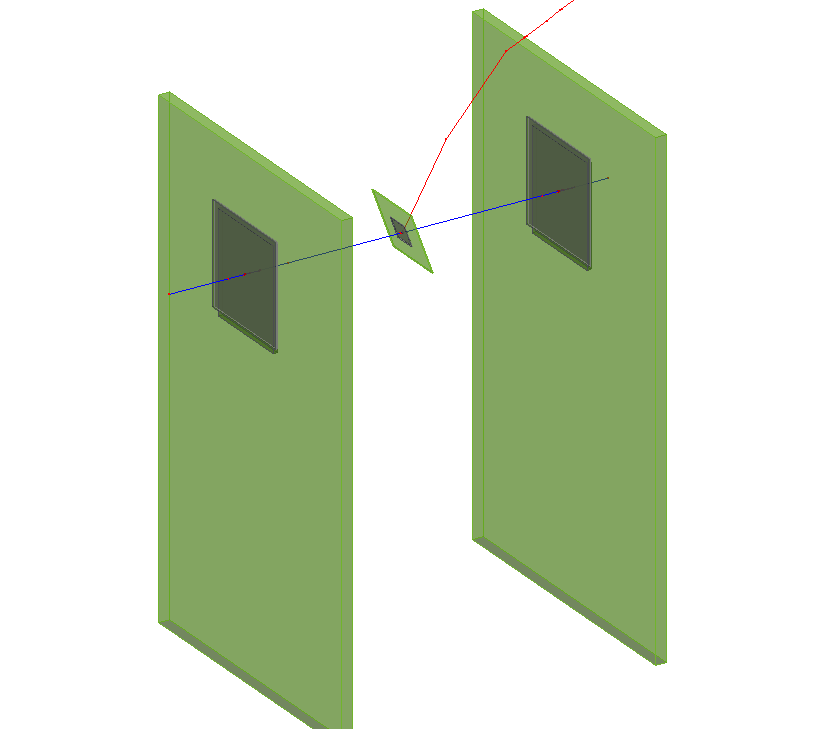
\includegraphics[width=0.6\textwidth]{telescope.png}
  \caption{Visualization of a Pion passing through the telescope setup defined in the detector configuration file. A secondary particle is produced in the material of the detector in the center.}
  \label{fig:telescope}
\end{figure}

An example configuration file describing a setup with one CLICpix2 detector and two Timepix~\cite{timepix} models is the following:
\inputminted[frame=single,framesep=3pt,breaklines=true,tabsize=2,linenos]{ini}{../../etc/manual_detector.conf}
Figure~\ref{fig:telescope} shows a visualization of the setup described in the file.
This configuration is used in the rest of this chapter for explaining concepts.

\subsubsection{Passive material configuration}
\label{sec:passive_material_config}

Descriptions of passive materials can be added to the detector setup via a set of sections, with a syntax similar to the detector configuration.
Passive geometry entries are identified by the \parameter{role} parameter set to \parameter{passive}.
Each section starts with a header describing the name used to identify the passive material; all names are required to be unique.

Every passive material has to contain all of the following parameters:
\begin{itemize}
  \item The \parameter{position} and \parameter{orientation} of the material as described for the detector, see Section \ref{sec:detector_config}.
  \item A string referring to the \parameter{type} of the passive material. 
  The model should be interpreted by the module constructing the passive material, such as for example the GeometryBuilderGeant4 module.
  \item A string referring to the \parameter{material} of the passive material. 
  The materials are defined in the GeometryBuilderGeant4 module and are described in the module section.
  Note: If the material is the same as the material of its \parameter{mother_volume}, the passive material will not be shown in the visualization. In the case that the material is the same as the material of the world frame, the material will have a white colour instead of the default blue in the visualisation.
  \item A set of size parameters specific for the model that is chosen. 
  All size parameters that describe the total length of something are placed such that half of this total length extends from each side of the given \parameter{position}.
  If a parameter describes the radius, this means the radius will extend from the \parameter{position} on both sides, making its total size two times the radius in the given direction.
  The size parameters for the specific models are described in Section~\ref{geometrybuildergeant4}.
\end{itemize}

In addition, an optional string referring to the \parameter{mother_volume}, which defines another passive material the volume will be placed in, can be specified.
Note: If a mother volume is chosen, the position defined in the configuration file will be relative to the center of the mother volume. An error will be given if the specified mother volume is too small for the specified size or position of this volume. Per default, the mother volume is the world frame.
Note: if the \parameter{mother_volume} is a hollow material, only the non-hollow part of the material is considered part of the material. Placing a passive volume in the hollow part requires a different \parameter{mother_volume}.

Similar to the detector configuration, the parameters \parameter{orientation_mode} (see Section~\ref{sec:models_geometry}), \parameter{alignment_precision_position} and \parameter{alignment_precision_orientation} (see Section~\ref{sec:detector_config}) can be used optionally to define the rotation order and a possible misalignment of passive materials.

An example configuration file describing a set of passive materials with different configuration options is the following:
\inputminted[frame=single,framesep=3pt,breaklines=true,tabsize=2,linenos]{ini}{../../etc/manual_passive_materials.conf}
Figure~\ref{fig:passivematerials} shows a visualization of the setup described in the file.

\begin{figure}[t]
  \centering
  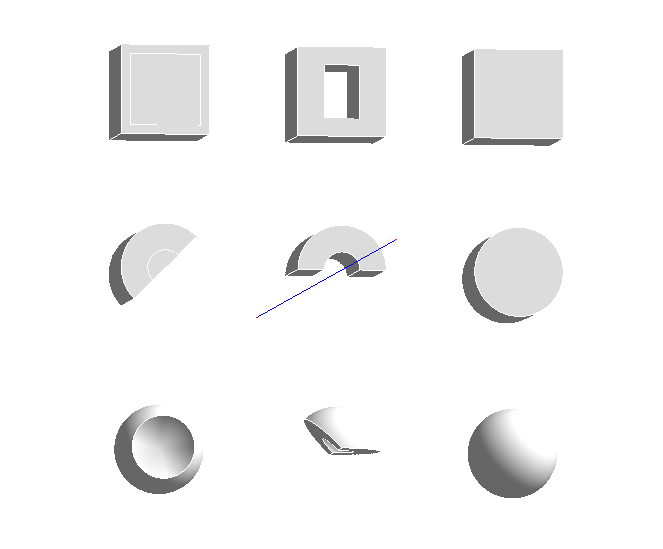
\includegraphics[width=0.6\textwidth]{passive_materials.png}
  \caption{Visualization of a set of passive materials showing different configuration options.}
  \label{fig:passivematerials}
\end{figure}


\section{Framework parameters}
\label{sec:framework_parameters}
The \apsq framework provides a set of global parameters which control and alter its behavior:
\begin{itemize}
\item \parameter{detectors_file}: Location of the file describing the detector configuration (introduced in Section~\ref{sec:detector_config}).
The only \textit{required} global parameter: the framework will fail to start if it is not specified.
\item \parameter{number_of_events}: Determines the total number of events the framework should simulate.
Defaults to one (simulating a single event).
\item \parameter{root_file}: Location relative to the \parameter{output_directory} where the ROOT output data of all modules will be written to. The file extension \texttt{.root} will be appended if not present.
Default value is \textit{modules.root}.
Directories within the ROOT file will be created automatically for all module instantiations.
\item \parameter{log_level}: Specifies the lowest log level which should be reported.
Possible values are \texttt{FATAL}, \texttt{STATUS}, \texttt{ERROR}, \texttt{WARNING}, \texttt{INFO} and \texttt{DEBUG}, where all options are case-insensitive.
Defaults to the \texttt{INFO} level.
More details and information about the log levels, including how to change them for a particular module, can be found in Section~\ref{sec:logging_verbosity}.
Can be overwritten by the \texttt{-v} parameter on the command line (see Section~\ref{sec:allpix_executable}).
\item \parameter{log_format}: Determines the log message format to display.
Possible options are \texttt{SHORT}, \texttt{DEFAULT} and \texttt{LONG}, where all options are case-insensitive.
More information can be found in Section~\ref{sec:logging_verbosity}.
\item \parameter{log_file}: File where the log output should be written to in addition to printing to the standard output (usually the terminal).
Only writes to standard output if this option is not provided.
Another (additional) location to write to can be specified on the command line using the \texttt{-l} parameter (see Section~\ref{sec:allpix_executable}).
\item \parameter{output_directory}: Directory to write all output files into.
Subdirectories are created automatically for all module instantiations.
This directory will also contain the \parameter{root_file} specified via the parameter described above.
Defaults to the current working directory with the subdirectory \textit{output/} attached.
\item \parameter{purge_output_directory}: Decides whether the content of an already existing output directory is deleted before a new run starts. Defaults to \texttt{false}, i.e. files are kept but will be overwritten by new files created by the framework.
\item \parameter{deny_overwrite}: Forces the framework to abort the run and throw an exception when attempting to overwrite an existing file. Defaults to \texttt{false}, i.e. files are overwritten when requested. This setting is inherited by all modules, but can be overwritten in the configuration section of each of the modules.
\item \parameter{random_seed}: Seed for the global random seed generator used to initialize seeds for module instantiations.
The 64-bit Mersenne Twister \command{mt19937_64} from the \CPP Standard Library is used to generate seeds.
A random seed from multiple entropy sources will be generated if the parameter is not specified.
Can be used to reproduce an earlier simulation run.
\item \parameter{random_seed_core}: Optional seed used for pseudo-random number generators in the core components of the framework. If not set explictely, the value $(\textrm{\parameter{random_seed}} + 1)$ is used.
\item \parameter{library_directories}: Additional directories to search for module libraries, before searching the default paths.
See Section~\ref{sec:module_instantiation} for details.
\item \parameter{model_paths}: Additional files or directories from which detector models should be read besides the standard search locations.
Refer to Section~\ref{sec:detector_models} for more information.
\item \parameter{experimental_multithreading}: Enable \textbf{experimental} multi-threading for the framework. This can speed up simulations of multiple detectors significantly. More information about multi-threading can be found in Section~\ref{sec:multithreading}.
\item \parameter{workers}: Specify the number of workers to use in total, should be strictly larger than zero. Only used if \parameter{experimental_multithreading} is set to true. Defaults to the number of native threads available on the system if this can be determined, otherwise one thread is used.
\end{itemize}

\section{The \textit{allpix} Executable}
\label{sec:allpix_executable}
The \parameter{allpix} executable functions as the interface between the user and the framework. It is primarily used to provide the main configuration file, but also allows to add and overwrite options from the main configuration file. This is both useful for quick testing as well as for batch processing of simulations.

The executable handles the following arguments:
\begin{itemize}
\item \texttt{-c <file>}: Specifies the configuration file to be used for the simulation, relative to the current directory.
This is the only \underline{required} argument, the simulation will fail to start if this argument is not given.
\item \texttt{-l <file>}: Specify an additional location to forward log output to, besides standard output and the location specified in the framework parameters explained in Section~\ref{sec:framework_parameters}.
\item \texttt{-v <level>}: Sets the global log verbosity level, overwriting the value specified in the configuration file described in Section~\ref{sec:framework_parameters}.
Possible values are \texttt{FATAL}, \texttt{STATUS}, \texttt{ERROR}, \texttt{WARNING}, \texttt{INFO} and \texttt{DEBUG}, where all options are case-insensitive.
The module specific logging level introduced in Section~\ref{sec:logging_verbosity} is not overwritten.
\item \texttt{-{}-version}: Prints the version and build time of the executable and terminates the program.
\item \texttt{-o <option>}: Passes extra framework or module options which are added and overwritten in the main configuration file.
This argument may be specified multiple times, to add multiple options.
Options are specified as key/value pairs in the same syntax as used in the configuration files (refer to Section~\ref{sec:config_file_format} for more details), but the key is extended to include a reference to a configuration section or instantiation in shorthand notation.
There are three types of keys that can be specified:
\begin{itemize}
\item Keys to set \textbf{framework parameters}. These have to be provided in exactly the same way as they would be in the main configuration file (a section does not need to be specified). An example to overwrite the standard output directory would be \texttt{allpix -c <file> -o output\_directory="run123456"}.
\item Keys for \textbf{module configurations}. These are specified by adding a dot (\texttt{.}) between the module and the actual key as it would be given in the configuration file (thus \textit{module}.\textit{key}). An example to overwrite the deposited particle to a positron would be \texttt{allpix -c <file> -o DepositionGeant4.particle\_type="e+"}.
\item Keys to specify values for a particular \textbf{module instantiation}. The identifier of the instantiation and the name of the actual key are split by a dot (\texttt{.}), in the same way as for keys for module configurations (thus \textit{identifier}.\textit{key}). The unique identifier for a module can contains one or more colons (\texttt{:}) to distinguish between various instantiations of the same module. The exact name of an identifier depends on the name of the detector and the optional input and output name. Those identifiers can be extracted from the logging section headers. An example to change the temperature of propagation for a particular instantiation for a detector named \textit{dut} could be \texttt{allpix -c <file> -o GenericPropagation:dut.temperature=273K}.
\end{itemize}
Note that only the single argument directly following the \texttt{-o} is interpreted as the option. If there is whitespace in the key/value pair this should be properly enclosed in quotation marks to ensure the argument is parsed correctly.
\item \texttt{-g <option>}: Passes extra detector options which are added and overwritten in the detector configuration file.
This argument can be specified multiple times, to add multiple options.
The options are parsed in the same way as described above for module options, but only one type of key can be specified to overwrite an option for a single detector.
These are specified by adding a dot (\texttt{.}) between the detector and the actual key as it would be given in the detector configuration file (thus \textit{detector}.\textit{key}). This method also works for customizing detector models as described in Section \ref{sec:detector_models}. An example to overwrite the sensor thickness for a particular detector named \texttt{detector1} to \texttt{50um} would be \texttt{allpix -c <file> -g detector1.sensor\_thickness=50um}.
\end{itemize}

No interaction with the framework is possible during the simulation. Signals can however be send using keyboard shortcuts to terminate the simulation, either gracefully or with force. The executable understand the following signals:
\begin{itemize}
    \item SIGINT (\texttt{CTRL+C}): Request a graceful shutdown of the simulation. This means the current simulated event is finished, while all other events requested in the configuration file are ignored. After finishing the event, the finalization stage is run for every module to ensure all modules finish properly. This signal can be very useful when too many events are specified and the simulation takes too long to finish entirely, but the output generated so far should still be kept.
    \item SIGTERM: Same as SIGINT, request a graceful shutdown of the simulation. This signal is emitted e.g.\ by the \command{kill} command or by cluster computing schedulers to ask for a termination of the job.
    \item SIGQUIT (\texttt{CTRL+\textbackslash}): Forcefully terminates the simulation. It is not recommmended to use this signal as it will normally lead to the loss of all generated data. This signal should only be used when graceful termination is for any reason not possible.
\end{itemize}


\section{Setting up the Simulation Chain}
\label{sec:setting_up_simulation_chain}

In the following, the framework parameters are used to set up a fully functional simulation.
Module parameters are shortly introduced when they are first used.
For more details about these parameters, the respective module documentation in Chapter~\ref{ch:modules} should be consulted.
A typical simulation in \apsq will contain the following components:
\begin{itemize}

\item The \textbf{geometry builder}, responsible for creating the external Geant4 geometry from the internal geometry.
In this document, \emph{internal geometry} refers to the detector parameters used by \apsq for coordinate transformations and conversions throughout the simulation, while \emph{external geometry} refers to the constructed Geant4 geometry used for charge carrier deposition (and possibly visualization).
\item The \textbf{deposition} module that simulates the particle beam creating charge carriers in the detectors using the provided physics list (containing a description of the simulated interactions) and the geometry created above.
\item A \textbf{propagation} module that propagates the charges through the sensor.
\item A \textbf{transfer} module that transfers the charges from the sensor electrodes and assigns them to a pixel of the readout electronics.
\item A \textbf{digitizer} module which converts the charges in the pixel to a detector hit, simulating the front-end electronics response.
\item An \textbf{output} module, saving the data of the simulation.
The \apsq standard file format is a ROOT TTree, which is described in detail in Section~\ref{sec:storing_output_data}.
\end{itemize}

In this example, charge carriers will be deposited in the three sensors defined in the detector configuration file in Section~\ref{sec:detector_config}.
All charge carriers deposited in the different sensors will be propagated and digitized.
Finally, monitoring histograms for the device under test (DUT) will be recorded in the framework's main ROOT file and all simulated objects, including the entry and exit positions of the simulated particles (Monte Carlo truth), will be stored in a ROOT file using the \apsq format.
An example configuration file implementing this would look like:
\inputminted[frame=single,framesep=3pt,breaklines=true,tabsize=2,linenos]{ini}{../../etc/manual.conf}

This configuration is available in the repository at \file{etc/manual.conf}.
The detector configuration file from Section~\ref{sec:detector_config} can be found at \file{etc/manual_detector.conf}.

The simulation is started by passing the path of the main configuration file to the \parameter{allpix} executable as follows:
\begin{verbatim}
$ allpix -c etc/manual.conf
\end{verbatim}
The detector histograms such as the hit map are stored in the ROOT file \file{output/modules.root} in the TDirectory \textit{DetectorHistogrammer/}.

If problems occur when exercising this example, it should be made sure that an up-to-date and properly installed version of \apsq is used (see the installation instructions in Chapter~\ref{ch:installation}).
If modules or models fail to load, more information about potential issues with the library loading can be found in the detailed framework description in Chapter~\ref{ch:framework}.

\section{Extending the Simulation Chain}
In the following, a few basic modules will be discussed which may be of use during a first simulation.

\paragraph{Visualization}
Displaying the geometry and the particle tracks helps both in checking and interpreting the results of a simulation.
Visualization is fully supported through Geant4, supporting all the options provided by Geant4~\cite{geant4vis}.
Using the Qt viewer with OpenGL driver is the recommended option as long as the installed version of Geant4 is built with Qt support enabled.

To add the visualization, the \parameter{VisualizationGeant4} section should be added at the end of the configuration file.
An example configuration with some useful parameters is given below:
\begin{minted}[frame=single,framesep=3pt,breaklines=true,tabsize=2,linenos]{ini}
[VisualizationGeant4]
# Use the Qt gui
mode = "gui"

# Set transparency of the detector models (in percent)
transparency = 0.4
# Set viewing style (alternative is 'wireframe')
view_style = "surface"

# Color trajectories by charge of the particle
trajectories_color_mode = "charge"
trajectories_color_positive = "blue"
trajectories_color_neutral = "green"
trajectories_color_negative = "red"
\end{minted}
If Qt is not available, a VRML viewer can be used as an alternative, however it is recommended to reinstall Geant4 with the Qt viewer included as it offers the best visualization capabilities.
The following steps are necessary in order to use a VRML viewer:
\begin{itemize}
\item A VRML viewer should be installed on the operating system.
Good options are FreeWRL or OpenVRML.
\item Subsequently, two environmental parameters have to be exported to the shell environment to inform Geant4 about the configuration:
\parameter{G4VRMLFILE_VIEWER} should point to the location of the viewer executable and \parameter{G4VRMLFILE_MAX_FILE_NUM} should typically be set to 1 to prevent too many files from being created.
\item Finally, the configuration section of the visualization module should be altered as follows:
\end{itemize}

\begin{minted}[frame=single,framesep=3pt,breaklines=true,tabsize=2,linenos]{ini}
[VisualizationGeant4]
# Do not start the Qt gui
mode = "none"
# Use the VRML driver
driver = "VRML2FILE"
\end{minted}

More information about all possible configuration parameters can be found in the module documentation in Chapter~\ref{ch:modules}.

\paragraph{Electric Fields}
\label{sec:module_electric_field}
By default, detectors do not have an electric field associated with them, and no bias voltage is applied.
A field can be added to each detector using the \parameter{ElectricFieldReader} module.

The section below calculates a linear electric field for every point in active sensor volume based on the depletion voltage of the sensor and the applied bias voltage.
The sensor is always depleted from the implant side; the direction of the electric field depends on the sign of the bias voltage as described in the module description in Chapter~\ref{ch:modules}.
\begin{minted}[frame=single,framesep=3pt,breaklines=true,tabsize=2,linenos]{ini}
# Add an electric field
[ElectricFieldReader]
# Set the field type to `linear`
model = "linear"
# Applied bias voltage to calculate the electric field from
bias_voltage = -50V
# Depletion voltage at which the given sensor is fully depleted
depletion_voltage = -10V
\end{minted}

\apsq also provides the possibility to utilize a full electrostatic TCAD simulation for the description of the electric field.
In order to speed up the lookup of the electric field values at different positions in the sensor, the adaptive TCAD mesh has to be interpolated and transformed into a regular grid with configurable feature size before use.
\apsq comes with a converter tool which reads TCAD DF-ISE files from the sensor simulation, interpolates the field, and writes this out in an appropriate format.
A more detailed description of the tool can be found in Section~\ref{sec:tcad_electric_field_converter}.
An example electric field (with the file name used in the example below) can be found in the \textit{etc} directory of the \apsq repository.

Electric fields can be attached to a specific detector using the standard syntax for detector binding.
A possible configuration would be:
\begin{minted}[frame=single,framesep=3pt,breaklines=true,tabsize=2,linenos]{ini}
[ElectricFieldReader]
# Bind the electric field to the detector named `dut`
name = "dut"
# Specify that the model is provided as meshed electric field map format, e.g. converted from TCAD
model = "mesh"
# Name of the file containing the electric field
file_name = "example_electric_field.init"
\end{minted}

\paragraph{Magnetic Fields}
\label{sec:module_magnetic_field}

For simulating the detector response in the presence of a magnetic field with \apsq, a constant, global magnetic field can be defined. By default, it is turned off. A field can be added to the whole setup using the unique module \parameter{MagneticFieldReader}, passing the field vector as parameter:
\begin{minted}[frame=single,framesep=3pt,breaklines=true,tabsize=2,linenos]{ini}
# Add a magnetic field
[MagneticFieldReader]
# Constant magnetic field (currently this is the default value)
model="constant"
# Magnetic field vector
magnetic_field = 0mT 3.8T 0T
\end{minted}

The global magnetic field is used by the interface to Geant4 and therefore exposes charged primary particles to the Lorentz force, and as a property of each detector present, enabling a Lorentz drift of the charge carriers in the active sensors, if supported by the used propagation modules. See Chapter \ref{ch:modules} for more information on the available propagation modules.

Currently, only constant magnetic fields can be applied.

\section{Logging and Verbosity Levels}
\label{sec:logging_verbosity}
\apsq is designed to identify mistakes and implementation errors as early as possible and to provide the user with clear indications about the problem.
The amount of feedback can be controlled using different log levels which are inclusive, i.e.\ lower levels also include messages from all higher levels.
The global log level can be set using the global parameter \parameter{log_level}.
The log level can be overridden for a specific module by adding the \parameter{log_level} parameter to the respective configuration section.
The following log levels are supported:
\begin{itemize}
\item \textbf{FATAL}: Indicates a fatal error that will lead to direct termination of the application.
Typically only emitted in the main executable after catching exceptions as they are the preferred way of fatal error handling (as discussed in Section~\ref{sec:error_reporting_exceptions}).
An example of a fatal error is an invalid configuration parameter.
\item \textbf{STATUS}: Important information about the status of the simulation.
Is only used for messages which have to be logged in every run such as the global seed for pseudo-random number generators and the current progress of the run.
\item \textbf{ERROR}: Severe error that should not occur during a normal well-configured simulation run.
Frequently leads to a fatal error and can be used to provide extra information that may help in finding the problem (for example used to indicate the reason a dynamic library cannot be loaded).
\item \textbf{WARNING}: Indicate conditions that should not occur normally and possibly lead to unexpected results.
The framework will however continue without problems after a warning.
A warning is for example issued to indicate that an output message is not used and that a module may therefore perform unnecessary work.
\item \textbf{INFO}: Information messages about the physics process of the simulation.
Contains summaries of the simulation details for every event and for the overall simulation.
Should typically produce maximum one line of output per event and module.
\item \textbf{DEBUG}: In-depth details about the progress of the simulation and all physics details of the simulation.
Produces large volumes of output per event, and should therefore only be used for  debugging the physics simulation of the modules.
\item \textbf{TRACE}: Messages to trace what the framework or a module is currently doing.
Unlike the \textbf{DEBUG} level, it does not contain any direct information about the physics of the simulation but rather indicates which part of the module or framework is currently running.
Mostly used for software debugging or determining performance bottlenecks in the simulations.
\end{itemize}

\begin{warning}
    It is not recommended to set the \parameter{log_level} higher than \textbf{WARNING} in a typical simulation as important messages may be missed.
    Setting too low logging levels should also be avoided since printing many log messages will significantly slow down the simulation.
\end{warning}

The logging system supports several formats for displaying the log messages.
The following formats are supported via the global parameter \parameter{log_format} or the individual module parameter with the same name:
\begin{itemize}
\item \textbf{SHORT}: Displays the data in a short form.
Includes only the first character of the log level followed by the configuration section header and the message.
\item \textbf{DEFAULT}: The default format.
Displays system time, log level, section header and the message itself.
\item \textbf{LONG}: Detailed logging format.
Displays all of the above but also indicates source code file and line where the log message was produced.
This can help in debugging modules.
\end{itemize}

More details about the logging system and the procedure for reporting errors in the code can be found in Sections~\ref{sec:logger} and~\ref{sec:error_reporting_exceptions}.

\section{Storing Output Data}
\label{sec:storing_output_data}
Storing the simulation output to persistent storage is of primary importance for subsequent reprocessing and analysis.
\apsq primarily uses ROOT for storing output data, given that it is a standard tool in High-Energy Physics and allows objects to be written directly to disk.
The \parameter{ROOTObjectWriter} automatically saves all objects created in a TTree~\cite{roottree}.
It stores separate trees for all object types and creates branches for every unique message name: a combination of the detector, the module and the message output name as described in Section~\ref{sec:redirect_module_input_outputs}.
For each event, values are added to the leaves of the branches containing the data of the objects.
This allows for easy histogramming of the acquired data over the total run using standard ROOT utilities.

Relations between objects within a single event are internally stored as ROOT TRefs~\cite{roottref}, allowing retrieval of related objects as long as these are loaded in memory.
An exception will be thrown when trying to access an object which is not in memory.
Refer to Section~\ref{sec:objhistory} for more information about object history.

In order to save all objects of the simulation, a \parameter{ROOTObjectWriter} module has to be added with a \parameter{file_name} parameter to specify the file location of the created ROOT file in the global output directory.
The file extension \texttt{.root} will be appended if not present.
The default file name is \texttt{data}, i.e.\ the file \textbf{data.root} is created in the output directory.
To replicate the default behaviour the following configuration can be used:
\begin{minted}[frame=single,framesep=3pt,breaklines=true,tabsize=2,linenos]{ini}
# The object writer listens to all output data
[ROOTObjectWriter]
# specify the output file (default file name is used if omitted)
file_name = "data"
\end{minted}
The generated output file can be analyzed using ROOT macros.
A simple macro for converting the results to a tree with standard branches for comparison is described in Section~\ref{sec:root_analysis_macros}.

It is also possible to read object data back in, in order to dispatch them as messages to further modules.
This feature is intended to allow splitting the execution of parts of the simulation into independent steps, which can be repeated multiple times.
The tree data can be read using a \parameter{ROOTObjectReader} module, which automatically dispatches all objects to the correct module instances.
An example configuration for using this module is:
\begin{minted}[frame=single,framesep=3pt,breaklines=true,tabsize=2,linenos]{ini}
# The object reader dispatches all objects in the tree
[ROOTObjectReader]
# path to the output data file, absolute or relative to the configuration file
file_name = "../output/data.root"
\end{minted}

The \apsq framework comes with a few more output modules which allow data storage in different formats, such as the LCIO persistency event data model~\cite{lcio}, the native RCE file format~\cite{rce}, or the Corryvreckan reconstruction framework data format.
Detailed descriptions of these modules can be found in Chapter~\ref{ch:modules}.


% core framework
\chapter{Structure \& Components of the Framework}
\label{ch:framework}

This chapter details the technical implementation of the \apsq framework and is mostly intended to provide insight into the gearbox to potential developers and interested users.
The framework consists of the following four main components that together form \apsq:
\begin{enumerate}
\item \textbf{Core}: The core contains the internal logic to initialize the modules, provide the geometry, facilitate module communication and run the event sequence.
The core keeps its dependencies to a minimum (it only relies on ROOT) and remains independent from the other components as far as possible.
It is the main component discussed in this section.
\item \textbf{Modules}: A module is a set of methods which is executed as part of the simulation chain.
Modules are built as separate libraries and loaded dynamically on demand by the core.
The available modules and their parameters are discussed in detail in Chapter~\ref{ch:modules}.
\item \textbf{Objects}: Objects form the data passed between modules using the message framework provided by the core.
Modules can listen and bind to messages with objects they wish to receive.
Messages are identified by the object type they are carrying, but can also be renamed to allow the direction of data to specific modules, facilitating more sophisticated simulation setups.
Messages are intended to be read-only and a copy of the data should be made if a module wishes to change the data.
All objects are compiled into a separate library which is automatically linked to every module.
More information about the messaging system and the supported objects can be found in Section~\ref{sec:objects_messages}.
\item \textbf{Tools}: \apsq provides a set of header-only 'tools' and a shared library that allow access to common logic shared by various modules.
Examples are the Runge-Kutta solver~\cite{fehlberg} implemented using the Eigen3 library and the set of template specializations for ROOT and Geant4 configurations.
More information about the tools can be found in Chapter~\ref{ch:additional_tools_resources}.
This set of tools is different from the set of core utilities the framework itself provides, which is part of the core and explained in Section~\ref{sec:logging_utilities}.
\end{enumerate}
Finally, \apsq provides an executable which instantiates the core of the framework, receives and distributes the configuration object and runs the simulation chain.

The chapter is structured as follows.
Section~\ref{sec:arch} provides an overview of the architectural design of the core and describes its interaction with the rest of the \apsq framework.
The different subcomponents such as configuration, modules and messages are discussed in Sections~\ref{sec:config_parameters}--\ref{sec:objects_messages}.
The chapter closes with a description of the available framework tools in Section~\ref{sec:logging_utilities}.
Some \CPP code will be provided in the text, but readers not interested may skip the technical details.

\section{Architecture of the Core}
\label{sec:arch}
The core is constructed as a light-weight framework which provides various subsystems to the modules.
It contains the part of the software responsible for instantiating and running the modules from the supplied configuration file, and is structured around five subsystems, of which four are centered around a manager and the fifth contains a set of general utilities.
The systems provided are:
\begin{enumerate}
\item \textbf{Configuration}: The configuration subsystem provides a configuration object from which data can be retrieved or stored, together with a TOML-like~\cite{tomlgit} parser to read configuration files.
It also contains the \apsq configuration manager which provides access to the main configuration file and its sections.
It is used by the module manager system to find the required instantiations and access the global configuration.
More information is given in Section~\ref{sec:config_parameters}.
\item \textbf{Module}: The module subsystem contains the base class of all \apsq modules as well as the manager responsible for loading and executing the modules (using the configuration system).
This component is discussed in more detail in Section~\ref{sec:module_manager}.
\item \textbf{Geometry}: The geometry subsystem supplies helpers for the simulation geometry.
The manager instantiates all detectors from the detector configuration file.
A detector object contains the position and orientation linked to an instantiation of a particular detector model, itself containing all parameters describing the geometry of the detector.
More details about geometry and detector models is provided in Section~\ref{sec:models_geometry}.
\item \textbf{Messenger}: The messenger is responsible for sending objects from one module to another.
The messenger object is passed to every module and can be used to bind to messages to listen for.
Messages with objects are also dispatched through the messenger as described in Section~\ref{sec:objects_messages}.
\item \textbf{Utilities}: The framework provides a set of utilities for logging, file and directory access, and unit conversion.
An explanation on how to use of these utilities can be found in Section~\ref{sec:logging_utilities}.
A set of \CPP exceptions is also provided in the utilities, which are inherited and extended by the other components.
Proper use of exceptions, together with logging information and reporting errors, makes the framework easier to use and debug.
A few notes about the use and structure of exceptions are provided in Section~\ref{sec:error_reporting_exceptions}.
\end{enumerate}

\section{Configuration and Parameters}
\label{sec:config_parameters}
Individual modules as well as the framework itself are configured through configuration files, which all follow the same format.
Explanations on how to use the various configuration files together with several examples have been provided in Section~\ref{sec:configuration_files}.

\subsection{File format}
\label{sec:config_file_format}
Throughout the framework, a simplified version of TOML~\cite{tomlgit} is used as standard format for configuration files.
The format is defined as follows:
\begin{enumerate}
\item All whitespace at the beginning or end of a line are stripped by the parser.
In the rest of this format specification the \textit{line} refers to the line with this whitespace stripped.
\item Empty lines are ignored.
\item Every non-empty line should start with either \texttt{\#}, \texttt{[} or an alphanumeric character.
Every other character should lead to an immediate parse error.
\item If the line starts with a hash character (\texttt{\#}), it is interpreted as comment and all other content on the same line is ignored.
\item If the line starts with an open square bracket (\texttt{[}), it indicates a section header (also known as configuration header).
The line should contain a string with alphanumeric characters and underscores, indicating the header name, followed by a closing square bracket (\texttt{]}), to end the header.
After any number of ignored whitespace characters there could be a \texttt{\#} character.
If this is the case, the rest of the line is handled as specified in point~3.
Otherwise there should not be any other character (except the whitespace) on the line.
Any line that does not comply to these specifications should lead to an immediate parse error.
Multiple section headers with the same name are allowed.
All key-value pairs following this section header are part of this section until a new section header is started.
\item If the line starts with an alphanumeric character, the line should indicate a key-value pair.
The beginning of the line should contain a string of alphabetic characters, numbers, dots (\texttt{.}), colons (\texttt{\:}) and underscores (\texttt{\_}), but it may only start with an alphanumeric character.
This string indicates the 'key'.
After an optional number of ignored whitespace, the key should be followed by an equality sign (\texttt{$=$}).
Any text between the \texttt{$=$} and the first \texttt{\#} character not enclosed within a pair of single or double quotes (\texttt{'} or \texttt{"}) is known as the non-stripped string.
Any character after the \texttt{\#} is handled as specified in point 3.
If the line does not contain any non-enclosed \texttt{\#} character, the value ends at the end of the line instead.
The 'value' of the key-value pair is the non-stripped string with all whitespace in front and at the end stripped.
The value may not be empty.
Any line that does not comply to these specifications should lead to an immediate parse error.
\item The value may consist of multiple nested dimensions which are grouped by pairs of square brackets (\texttt{[} and \texttt{]}).
The number of square brackets should be properly balanced, otherwise an error is raised.
Square brackets which should not be used for grouping should be enclosed in quotation marks.
Every dimension is split at every whitespace sequence and comma character (\texttt{,}) not enclosed in quotation marks.
Implicit square brackets are added to the begin and end of the value, if these are not explicitly added.
A few situations require explicit addition of outer brackets such as matrices with only one column element, i.e. with dimension 1xN.
\item The sections of the value which are interpreted as separate entities are named elements.
For a single value the element is on the zeroth dimension, for arrays on the first dimension and for matrices on the second dimension.
Elements can be forced by using quotation marks, either single or double quotes (\texttt{'} or \texttt{"}).
The number of both types of quotation marks should be properly balanced, otherwise an error is raised.
The conversion to the elements to the actual type is performed when accessing the value.
\item All key-value pairs defined before the first section header are part of a zero-length empty section header.
\end{enumerate}

\subsection{Accessing parameters}
\label{sec:accessing_parameters}
Values are accessed via the configuration object.
In the following example, the key is a string called \parameter{key}, the object is named \parameter{config} and the type \parameter{TYPE} is a valid \CPP type the value should represent.
The values can be accessed via the following methods:
\begin{minted}[frame=single,framesep=3pt,breaklines=true,tabsize=2,linenos]{c++}
// Returns true if the key exists and false otherwise
config.has("key")
// Returns the number of keys found from the provided initializer list:
config.count({"key1", "key2", "key3"});
// Returns the value in the given type, throws an exception if not existing or a conversion to TYPE is not possible
config.get<TYPE>("key")
// Returns the value in the given type or the provided default value if it does not exist
config.get<TYPE>("key", default_value)
// Returns an array of elements of the given type
config.getArray<TYPE>("key")
// Returns a matrix: an array of arrays of elements of the given type
config.getMatrix<TYPE>("key")
// Returns an absolute (canonical if it should exist) path to a file
config.getPath("key", true /* check if path exists */)
// Return an array of absolute paths
config.getPathArray("key", false /* do not check if paths exists */)
// Returns the value as literal text including possible quotation marks
config.getText("key")
// Set the value of key to the default value if the key is not defined
config.setDefault("key", default_value)
// Set the value of the key to the default array if key is not defined
config.setDefaultArray<TYPE>("key", vector_of_default_values)
// Create an alias named new_key for the already existing old_key or throws an exception if the old_key does not exist
config.setAlias("new_key", "old_key")
\end{minted}

Conversions to the requested type are using the \parameter{from_string} and \parameter{to_string} methods provided by the string utility library described in Section~\ref{sec:string_utilities}.
These conversions largely follow standard \CPP parsing, with one important exception.
If (and only if) the value is retrieved as a C/\CPP string and the string is fully enclosed by a pair of \texttt{"} characters, these are stripped before returning the value.
Strings can thus also be provided with or without quotation marks.

\begin{warning}
    It should be noted that a conversion from string to the requested type is a comparatively heavy operation.
    For performance-critical sections of the code, one should consider fetching the configuration value once and caching it in a local variable.
\end{warning}

\section{Modules and the Module Manager}
\label{sec:module_manager}
\apsq is a modular framework and one of the core ideas is to partition functionality in independent modules which can be inserted or removed as required.
These modules are located in the subdirectory \textit{src/modules/} of the repository, with the name of the directory the unique name of the module.
The suggested naming scheme is CamelCase, thus an example module name would be \textit{GenericPropagation}.
There are two different kind of modules which can be defined:
\begin{itemize}
    \item \textbf{Unique}: Modules for which a single instance runs, irrespective of the number of detectors.
    \item \textbf{Detector}: Modules which are concerned with only a single detector at a time.
    These are then replicated for all required detectors.
\end{itemize}
The type of module determines the constructor used, the internal unique name and the supported configuration parameters.
For more details about the instantiation logic for the different types of modules, see Section~\ref{sec:module_instantiation}.

\subsection{Module instantiation}
\label{sec:module_instantiation}
Modules are dynamically loaded and instantiated by the Module Manager.
They are constructed, initialized, executed and finalized in the linear order in which they are defined in the configuration file; for this reason the configuration file should follow the order of the real process.
For each section in the main configuration file (see~\ref{sec:config_parameters} for more details), a corresponding library is searched for which contains the module (the exception being the global framework section).
Module libraries are always named following the scheme \textbf{libAllpixModule\texttt{ModuleName}}, reflecting the \texttt{ModuleName} configured via CMake.
The module search order is as follows:
\begin{enumerate}
\item Modules already loaded before from an earlier section header
\item All directories in the global configuration parameter \parameter{library_directories} in the provided order, if this parameter exists.
\item The internal library paths of the executable, that should automatically point to the libraries that are built and installed together with the executable.
These library paths are stored in \dir{RPATH} on Linux, see the next point for more information.
\item The other standard locations to search for libraries depending on the operating system.
Details about the procedure Linux follows can be found in~\cite{linuxld}.
\end{enumerate}

If the loading of the module library is successful, the module is checked to determine if it is a unique or detector module.
As a single module may be called multiple times in the configuration, with overlapping requirements (such as a module which runs on all detectors of a given type, followed by the same module but with different parameters for one specific detector, also of this type) the Module Manager must establish which instantiations to keep and which to discard.
The instantiation logic determines a unique name and priority, where a lower number indicates a higher priority, for every instantiation.
The name and priority for the instantiation are determined differently for the two types of modules:
\begin{itemize}
\item \textbf{Unique}: Combination of the name of the module and the \parameter{input} and \parameter{output} parameter (both defaulting to an empty string).
The priority is always zero.
\item \textbf{Detector}: Combination of the name of the module, the \parameter{input} and \parameter{output} parameter (both defaulting to an empty string) and the name of detector this module is executed for.
If the name of the detector is specified directly by the \parameter{name} parameter, the priority is \emph{high}.
If the detector is only matched by the \parameter{type} parameter, the priority is \emph{medium}.
If the \parameter{name} and \parameter{type} are both unspecified and the module is instantiated for all detectors, the priority is \emph{low}.
\end{itemize}
In the end, only a single instance for every unique name is allowed.
If there are multiple instantiations with the same unique name, the instantiation with the highest priority is kept.
If multiple instantiations with the same unique name and the same priority exist, an exception is raised.

\subsection{Multithreading: Parallel execution of events}
\label{sec:multithreading}
The framework supports running several events in parallel via its multithreading feature.
By default, this feature is disabled for new modules.
If supported by all modules in the simulation, multithreading is enabled by default, but can be disabled by the user as described in Section~\ref{sec:framework_parameters}.
When enabled this feature can provide a significant speed improvement, depending on the simulation chain.

The framework allows to parallelize the execution of the same module for multiple events, if these would otherwise be executed directly after each other in a linear order.
Thus, events are added to a work queue and then distributed to a set of worker threads as specified in the configuration or determined from system parameters.

Detailed description of how the framework implements the multithreading feature can be found in Section~\ref{sec:multithreading_approach} and an overview of important considerations when writing a new module capable of multithreading is provided in Section~\ref{sec:module_multithreading}.

\section{Geometry and Detectors}
\label{sec:models_geometry}
Simulations are frequently performed for a set of different detectors (such as a beam telescope and a device under test).
All of these individual detectors together form what \apsq defines as the geometry.
Each detector has a set of properties attached to it:
\begin{itemize}
\item A unique detector \parameter{name} to refer to the detector in the configuration.
\item The \parameter{position} in the world frame.
This is the position of the geometric center of the sensitive device (sensor) given in world coordinates as X, Y and Z as defined in Section~\ref{sec:coordinate_systems} (note that any additional components like the chip and possible support layers are ignored when determining the geometric center).
\item An \parameter{orientation_mode} that determines the way that the orientation is applied.
This can be either \texttt{xyz}, \texttt{zyx} or \texttt{zxz}, where \textbf{\texttt{xyz} is used as default if the parameter is not specified}. Three angles are expected as input, which should always be provided in the order in which they are applied.
\begin{itemize}
    \item The \texttt{xyz} option uses extrinsic Euler angles to apply a rotation around the global $X$ axis, followed by a rotation around the global $Y$ axis and finally a rotation around the global $Z$ axis.
    \item The \texttt{zyx} option uses the \textbf{extrinsic Z-Y-X convention} for Euler angles, also known as Pitch-Roll-Yaw or 321 convention. The rotation is represented by three angles describing first a rotation of an angle $\phi$ (yaw) about the $Z$ axis, followed by a rotation of an angle $\theta$ (pitch) about the initial $Y$ axis, followed by a third rotation of an angle $\psi$ (roll) about the initial $X$ axis.
    \item The \texttt{zxz} uses the \textbf{extrinsic Z-X-Z convention} for Euler angles instead. This option is also known as the 3-1-3 or the "x-convention" and the most widely used definition of Euler angles~\cite{eulerangles}.
\end{itemize}
\begin{warning}
It is highly recommended to always explicitly state the orientation mode instead of relying on the default configuration.
\end{warning}

\item The \parameter{orientation} to specify the Euler angles in logical order (e.g. first $X$, then $Y$, then $Z$ for the \texttt{xyz} method), interpreted using the method above (or with the \texttt{xyz} method if the \parameter{orientation_mode} is not specified). An example for three Euler angles would be
\begin{minted}[frame=single,framesep=3pt,breaklines=true,tabsize=2,linenos]{ini}
orientation_mode = "zyx"
orientation = 45deg 10deg 12deg
\end{minted}
which describes the rotation of \SI{45}{\degree} around the $Z$ axis, followed by a \SI{10}{\degree} rotation around the initial $Y$ axis, and finally a rotation of \SI{12}{\degree} around the initial $X$ axis.
\begin{warning}
All supported rotations are extrinsic active rotations, i.e. the vector itself is rotated, not the coordinate system. All angles in configuration files should be specified in the order they will be applied.
\end{warning}

\item A \parameter{type} parameter describing the detector model, for example \emph{timepix} or \emph{mimosa26}.
These models define the geometry and parameters of the detector.
Multiple detectors can share the same model, several of which are shipped ready-to-use with the framework.
\item An optional parameter \parameter{alignment_precision_position} to specify the alignment precision along the three global axes as described in Section~\ref{sec:detector_config}.
\item An optional parameter \parameter{alignment_precision_orientation} for the alignment precision in the three rotation angles as described in Section~\ref{sec:detector_config}.
\item An optional \textbf{electric field} in the sensitive device.
An electric field can be added to a detector by a special module as demonstrated in Section~\ref{sec:module_electric_field}.
\end{itemize}
The detector configuration is provided in the detector configuration file as explained in Section~\ref{sec:detector_config}.

\subsection{Coordinate systems}
\label{sec:coordinate_systems}

Local coordinate systems for each detector and a global frame of reference for the full setup are defined.
The global coordinate system is chosen as a right-handed Cartesian system, and the rotations of individual devices are performed around the geometrical center of their sensor.

Local coordinate systems for the detectors are also right-handed Cartesian systems, with the x- and y-axes defining the sensor plane.
The origin of this coordinate system is the center of the lower left pixel in the grid, i.e.\ the pixel with indices (0,0).
This simplifies calculations in the local coordinate system as all positions can either be stated in absolute numbers or in fractions of the pixel pitch.

A sketch of the actual coordinate transformations performed, including the order of transformations, is provided in Figure~\ref{fig:transformations}. The global coordinate system used for tracking of particles through detetector setup is shown on the left side, while the local coordinate system used to describe the individual sensors is located at the right.

\begin{figure}[tbp]
  \center
  \tikzset{%
  >=latex
}
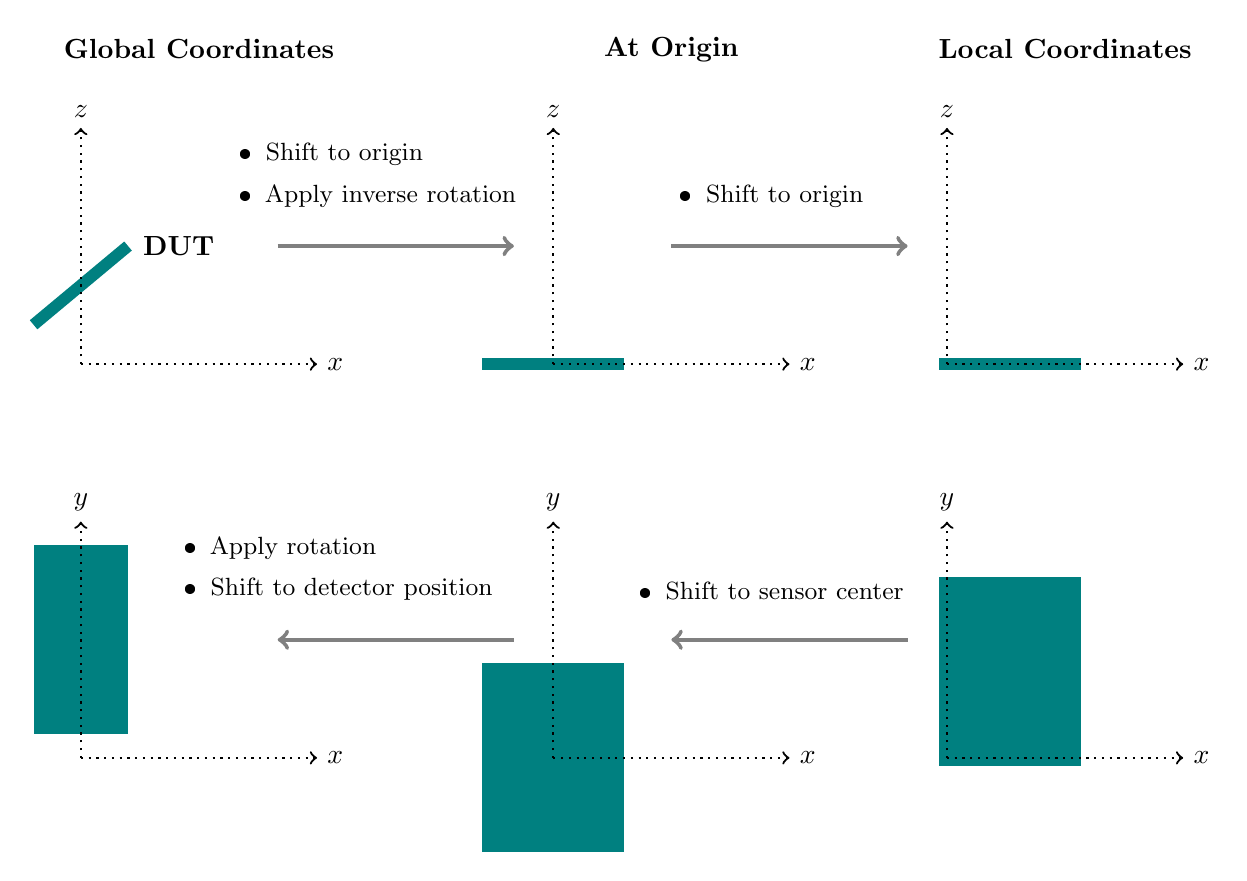
\begin{tikzpicture}

  % Labels
  \node[font=\bfseries] at (1.5,4) {Global Coordinates};
  \node[font=\bfseries] at (7.5,4) {At Origin};
  \node[font=\bfseries] at (12.5,4) {Local Coordinates};
  % \node[rotate=90,font=\bfseries] at (-1.5,1.5) {Top view};
  % \node[rotate=90,font=\bfseries] at (-1.5,-3.5) {Side view};

  % Detectors
  \draw [teal, line width=0.15cm] (-0.6, 0.5)  -- (0.6, 1.5) node [right,black] {\textbf{DUT}};
  \draw [teal, line width=0.15cm] (5.1, 0)  -- (6.9, 0);
  \draw [teal, line width=0.15cm] (10.9, 0)  -- (12.7, 0);

  \fill [teal] (-0.6,-4.7) rectangle (0.6,-2.3);
  \fill [teal] (5.1,-6.2) rectangle (6.9,-3.8);
  \fill [teal] (10.9,-5.1) rectangle (12.7,-2.7);

  % Explanations
  \draw [ultra thick, gray, ->] (2.5, 1.5) -- (3.5, 1.5) node [above, black, yshift=10] {
    \begin{varwidth}{\linewidth}
      \small
      \begin{itemize}
        \item Shift to origin
        \item Apply inverse rotation
      \end{itemize}
    \end{varwidth}
  } -- (5.5, 1.5);

  \draw [ultra thick, gray, ->] (7.5, 1.5) -- (8.5, 1.5) node [above, black, yshift=10] {
    \begin{varwidth}{\linewidth}
      \small
      \begin{itemize}
        \item Shift to origin
      \end{itemize}
    \end{varwidth}
  } -- (10.5, 1.5);

  \draw [ultra thick, gray, ->] (10.5, -3.5) -- (8.5, -3.5) node [above, black, yshift=10] {
    \begin{varwidth}{\linewidth}
      \small
      \begin{itemize}
        \item Shift to sensor center
      \end{itemize}
    \end{varwidth}
  } -- (7.5, -3.5);

  \draw [ultra thick, gray, ->] (5.5, -3.5) -- (3, -3.5) node [above, black, yshift=10] {
    \begin{varwidth}{\linewidth}
      \small
      \begin{itemize}
        \item Apply rotation
        \item Shift to detector position
      \end{itemize}
    \end{varwidth}
  } -- (2.5, -3.5);

  % Coordinates
  \draw [black, dotted, thick, ->] (0, 0) -- (0, 3) node [above] {$z$};
  \draw [black, dotted, thick, ->] (0, 0) -- (3, 0) node [right] {$x$};
  \draw [black, dotted, thick, ->] (6, 0) -- (6, 3) node [above] {$z$};
  \draw [black, dotted, thick, ->] (6, 0) -- (9, 0) node [right] {$x$};
  \draw [black, dotted, thick, ->] (11, 0) -- (11, 3) node [above] {$z$};
  \draw [black, dotted, thick, ->] (11, 0) -- (14, 0) node [right] {$x$};

  \draw [black, dotted, thick, ->] (0, -5) -- (0, -2) node [above] {$y$};
  \draw [black, dotted, thick, ->] (0, -5) -- (3, -5) node [right] {$x$};
  \draw [black, dotted, thick, ->] (6, -5) -- (6, -2) node [above] {$y$};
  \draw [black, dotted, thick, ->] (6, -5) -- (9, -5) node [right] {$x$};
  \draw [black, dotted, thick, ->] (11, -5) -- (11, -2) node [above] {$y$};
  \draw [black, dotted, thick, ->] (11, -5) -- (14, -5) node [right] {$x$};

\end{tikzpicture}

  \caption{Coordinate transformations from global to local and revers. The first row shows the detector positions in the respective coordinate systems in top view, the second row in side view.}
  \label{fig:transformations}
\end{figure}

The global reference for time measurements is the beginning of the event, i.e.\ the start of the particle tracking through the setup.
The local time reference is the time of entry of the \emph{first} primary particle of the event into the sensor.
This means that secondary particles created within the sensor inherit the local time reference from their parent particles in order to have a uniform time reference in the sensor.
It should be noted that Monte Carlo particles that start the local time frame on different detectors do not necessarily have to belong to the same particle track.

\subsection{Changing and accessing the geometry}
The geometry is needed at a very early stage because it determines the number of detector module instantiations as explained in Section~\ref{sec:module_instantiation}.
The procedure of finding and loading the appropriate detector models is explained in more detail in Section~\ref{sec:detector_models}.

The geometry is directly added from the detector configuration file described in Section~\ref{sec:detector_config}.
The geometry manager parses this file on construction, and the detector models are loaded and linked later during geometry closing as described above.
It is also possible to add additional models and detectors directly using \parameter{addModel} and \parameter{addDetector} (before the geometry is closed).
Furthermore it is possible to add additional points which should be part of the world geometry using \parameter{addPoint}.
This can for example be used to add the beam source to the world geometry.

The detectors and models can be accessed by name and type through the geometry manager using \parameter{getDetector} and \parameter{getModel}, respectively.
All detectors can be fetched at once using the \parameter{getDetectors} method.
If the module is a detector-specific module its related Detector can be accessed through the \parameter{getDetector} method of the module base class instead (returns a null pointer for unique modules) as follows:
\begin{minted}[frame=single,framesep=3pt,breaklines=true,tabsize=2,linenos]{c++}
void run(Event* event) {
    // Returns the linked detector
    std::shared_ptr<Detector> detector = this->getDetector();
}
\end{minted}

\subsection{Detector models}
\label{sec:detector_models}
Different types of detector models are available and distributed together with the framework: these models use the configuration format introduced in Section~\ref{sec:config_file_format} and can be found in the \textit{models} directory of the repository.
Every model extends from the \texttt{DetectorModel} base class, which defines the minimum required parameters of a detector model within the framework.
The coordinates place the detector in the global coordinate system, with the reference point taken as the geometric center of the active matrix.
This is defined by the number of pixels in the sensor in both the x- and y-direction, and together with the pitch of the individual pixels the total size of the pixel matrix is determined.
Outside the active matrix, the sensor can feature excess material in all directions in the x-y-plane.
A detector of base class type does not feature a separate readout chip, thus only the thickness of an additional, inactive silicon layer can be specified.
Derived models allow for separate readout chips, optionally connected with bump bonds.

The base detector model can be extended to provide more detailed geometries.
Currently implemented derived models are the \texttt{MonolithicPixelDetectorModel}, which describes a monolithic detector with all electronics directly implemented in the same silicon wafer as the sensor, and the \texttt{HybridPixelDetectorModel}, which in addition to the features described above also includes a separate readout chip with configurable size and bump bonds between the sensor and readout chip.

\nlparagraph{Detector model parameters}
Models are defined in configuration files which are used to instantiate the actual model classes; these files contain various types of parameters, some of which are required for all models while others are optional or only supported by certain model types.
For more details on how to add and use a new detector model, Section~\ref{sec:adding_detector_model} should be consulted.

The set of base parameters supported by every model is provided below.
These parameters should be given at the top of the file before the start of any sub-sections.
\begin{itemize}
\item \parameter{type}: A required parameter describing the type of the model.
At the moment either \parameter{monolithic} or \parameter{hybrid}.
This value determines the supported parameters as discussed later.
\item \parameter{number_of_pixels}: The number of pixels in the 2D pixel matrix.
Determines the base size of the sensor together with the \parameter{pixel_size} parameter below.
\item \parameter{pixel_size}: The pitch of a single pixel in the pixel matrix.
Provided as 2D parameter in the x-y-plane.
This parameter is required for all models.
\item \parameter{implant_size}: The size of the collection diode implant in each pixel of the matrix.
Provided as 2D parameter in the x-y-plane.
This parameter is optional, the implant size defaults to the pixel pitch if not specified otherwise.
\item \parameter{sensor_thickness}: Thickness of the active area of the detector model containing the individual pixels.
This parameter is required for all models.
\item \texttt{\textbf{sensor\_excess\_\textit{direction}}}: With direction either \parameter{top}, \parameter{bottom}, \parameter{right} or \parameter{left}, where the top, bottom, right and left direction are the positive y-axis, the negative y-axis, the positive x-axis and the negative x-axis, respectively.
Specifies the extra material added to the sensor outside the active pixel matrix in the given direction.
\item \parameter{sensor_excess}: Fallback for the excess width of the sensor in all four directions (top, bottom, right and left).
Used if the specialized parameters described below are not given.
Defaults to zero, thus having a sensor size equal to the number of pixels times the pixel pitch.
\item \parameter{chip_thickness}: Thickness of the readout chip, placed next to the sensor.
\end{itemize}

The base parameters described above are the only set of parameters supported by the \textbf{monolithic} model. For this model, the \parameter{chip_thickness} parameter represents the first few micrometers of silicon which contain the chip circuitry and are shielded from the bias voltage and thus do not contribute to the signal formation.

The \textbf{hybrid} model adds bump bonds between the chip and sensor while automatically making sure the chip and support layers are shifted appropriately.
Furthermore, it allows the user to specify the chip dimensions independently from the sensor size, as the readout chip is treated as a separate entity.
The additional parameters for the \textbf{hybrid} model are as follows:
\begin{itemize}
\item \texttt{\textbf{chip\_excess\_\textit{direction}}}: With direction either \parameter{top}, \parameter{bottom}, \parameter{right} or \parameter{left}.
The chip excess in the specific direction, similar to the \texttt{\textbf{sensor\_excess\_\textit{direction}}} parameter described above.
\item \parameter{chip_excess}: Fallback for the excess width of the chip, defaults to zero and thus to a chip size equal to the dimensions of the pixel matrix.
See the \parameter{sensor_excess} parameter above.
\item \parameter{bump_height}: Height of the bump bonds (the separation distance between the chip and the sensor)
\item \parameter{bump_sphere_radius}: The individual bump bonds are simulated as union solids of a sphere and a cylinder.
This parameter sets the radius of the sphere to use.
\item \parameter{bump_cylinder_radius}: The radius of the cylinder part of the bump.
The height of the cylinder is determined by the \parameter{bump_height} parameter.
\item \parameter{bump_offset}: A 2D offset of the grid of bumps.
The individual bumps are by default positioned at the center of each single pixel in the grid.
\end{itemize}


\nlparagraph{Support Layers}
\label{sec:support_layers}
In addition to the active layer, multiple layers of support material can be added to the detector description.
It is possible to place support layers at arbitrary positions relative to the sensor, while the default position is behind the readout chip (or inactive silicon layer).
The defined support materials will always be positioned relative to the corresponding detector.
The support material can be chosen from a set of predefined materials, including PCB and Kapton.

Every support layer should be defined in its own section headed with the name \texttt{[support]}.
By default, no support layers are added.
Support layers allow for the following parameters.
\begin{itemize}
\item \parameter{size}: Size of the support in 2D (the thickness is given separately below).
This parameter is required for all support layers.
\item \parameter{thickness}: Thickness of the support layers.
This parameter is required for all support layers.
\item \parameter{location}: Location of the support layer.
Either \textit{sensor} to attach it to the sensor (opposite to the readout chip/inactive silicon layer), \textit{chip} to add the support layer behind the chip/inactive layer or \textit{absolute} to specify the offset in the z-direction manually.
Defaults to \textit{chip} if not specified.
If the parameter is equal to \textit{sensor} or \textit{chip}, the support layers are stacked in the respective direction when multiple layers of support are specified.
\item \parameter{offset}: If the parameter \parameter{location} is equal to \textit{sensor} or \textit{chip}, an optional 2D offset can be specified using this parameter, the offset in the z-direction is then automatically determined.
These support layers are by default centered around the middle of the pixel matrix (the rotation center of the model).
If the \texttt{location} is set to \textit{absolute}, the offset is a required parameter and should be provided as a 3D vector with respect to the center of the model (thus the center of the active sensor).
Care should be taken to ensure that these support layers and the rest of the model do not overlap.
\item \parameter{hole_size}: Adds an optional cut-out hole to the support with the 2D size provided.
The hole always cuts through the full support thickness.
No hole will be added if this parameter is not present.
\item \parameter{hole_type}: Type of hole to be punched into the support layer. Currently supported are \textit{rectangle} and \textit{cylinder}. Defaults to \textit{rectangle}.
\item \parameter{hole_offset}: If present, the hole is by default placed at the center of the support layer.
A 2D offset with respect to its default position can be specified using this parameter.
\item \texttt{material}: Material of the support. \apsq does not provide a set of materials to choose from; it is up to the modules using this parameter to implement the materials such that they can use it.
Chapter~\ref{ch:modules} provides details about the materials supported by the geometry builder module (\parameter{GeometryBuilderGeant4}).
\todo{This should be standardized...}
\end{itemize}

\nlparagraph{Accessing specific detector models within the framework}
Some modules are written to act on only a particular type of detector model.
In order to ensure that a specific detector model has been used, the model should be downcast: the downcast returns a null pointer if the class is not of the appropriate type.
An example for fetching a \texttt{HybridPixelDetectorModel} would thus be:
\begin{minted}[frame=single,framesep=3pt,breaklines=true,tabsize=2,linenos]{c++}
// "detector" is a pointer to a Detector object
auto model = detector->getModel();
auto hybrid_model = std::dynamic_pointer_cast<HybridPixelDetectorModel>(model);
if(hybrid_model != nullptr) {
    // The model of this Detector is a HybridPixelDetectorModel
}
\end{minted}

\nlparagraph{Specializing detector models}
A detector model contains default values for all parameters.
Some parameters like the sensor thickness can however vary between different detectors of the same model.
To allow for easy adjustment of these parameters, models can be specialized in the detector configuration file introduced in~\ref{sec:detector_config}.
All model parameters, except the type parameter and the support layers, can be changed by adding a parameter with the exact same key and the updated value to the detector configuration.
The framework will then automatically create a copy of this model with the requested change.

\begin{warning}
Before re-implementing models, it should be checked if the desired change can be achieved using the detector model specialization. For most cases this provides a quick and flexible way to adapt detectors to different needs and setups (for example, detectors with different sensor thicknesses).
\end{warning}

\nlparagraph{Search order for models}
To support different detector models and storage locations, the framework searches different paths for model files in the following order:
\begin{enumerate}
\item If defined, the paths provided in the global \parameter{model_paths} parameter are searched first.
Files are read and parsed directly.
If the path is a directory, all files in the directory are added (without recursing into subdirectories).
\item The location where the models are installed to (refer to the description of the \parameter{MODEL_DIRECTORY} variable in Section~\ref{sec:cmake_config}).
\item The standard data paths on the system as given by the environmental variable \parameter{$XDG_DATA_DIRS} with ``\project/models'' appended.
The \parameter{$XDG_DATA_DIRS} variable defaults to \textit{/usr/local/share/} (thus effectively \textit{/usr/local/share/\project/models}) followed by \textit{/usr/share/} (effectively \textit{/usr/share/\project/models}).
\end{enumerate}

\section{Passing Objects using Messages}
\label{sec:objects_messages}
Communication between modules is performed by the exchange of messages.
Messages are templated instantiations of the \parameter{Message} class carrying a vector of objects.
The list of objects available in the \apsq objects library are discussed in Chapter~\ref{ch:objects}.
The messaging system has a dispatching mechanism to send messages and a receiving part that fetches incoming messages.
Messages are always received by modules in the order they have been dispatched by preceding modules.

The dispatching module can specify an optional name for the messages, but modules should normally not specify this name directly.
If the name is not given (or equal to \texttt{-}) the \parameter{output} parameter of the module is used to determine the name of the message, defaulting to an empty string.
Dispatching messages to their receivers is then performed following these rules:
\begin{enumerate}
    \item The receiving module will \underline{only} receive a message if it has the exact same type as the message dispatched (thus carrying the same objects).
    If the receiver is however listening to the \parameter{BaseMessage} type which does not specify the type of objects it is carrying, it will instead receive all dispatched messages.
    \item The receiving module will \underline{only} receive messages with the exact name it is listening for.
    The module uses the \parameter{input} parameter to determine which message names it should listen for; if the \parameter{input} parameter is equal to \texttt{*} the module will listen to all messages.
    Each module by default listens to messages with no name specified (thus receiving the messages of dispatching modules without output name specified).
    \item If the receiving module is a detector module, it will \underline{only} receive messages bound to that specific detector \underline{or} messages that are not bound to any detector.
\end{enumerate}

An example of how to dispatch a message containing an array of \parameter{Object} types bound to a detector named \texttt{dut} is provided below.
As usual, the message is dispatched at the end of the \parameter{run()} function of the module.
\begin{minted}[frame=single,framesep=3pt,breaklines=true,tabsize=2,linenos]{c++}
void run(Event* event) {
    std::vector<Object> data;
    // ..fill the data vector with objects ...

    // The message is dispatched only for the module's detector, stored in "detector_"
    auto message = std::make_shared<Message<Object>>(data, detector_);

    // Send the message using the Messenger object for the given event
    messenger->dispatchMessage(this, message, event);
}
\end{minted}

\subsection{Methods to process messages}
The message system has multiple methods to process received messages.
The first two are the most common methods and the third should be avoided in almost every instance.
\begin{enumerate}
\item Bind a \textbf{single message} to the input of this module.
This should usually be the preferred method, where a module expects only a single message to arrive per event containing the list of all relevant objects.
The following example binds to a message containing an array of objects and is placed in the constructor of a detector-type \parameter{TestModule}:
\begin{minted}[frame=single,framesep=3pt,breaklines=true,tabsize=2,linenos]{c++}
TestModule(Configuration&, Messenger* messenger, std::shared_ptr<Detector>) {
    // Subscribe to a single message, with no special messenger flags
    messenger->bindSingle<ExampleMessage>(this, MsgFlags::NONE);
}
\end{minted}
\item Bind a \textbf{set of messages} to the input of the module.
This method should be used if the module can (and expects to) receive the same message multiple times (possibly because it wants to receive the same type of message for all detectors).
An example to bind multiple messages containing an array of objects in the constructor of a unique-type \parameter{TestModule} would be:
\begin{minted}[frame=single,framesep=3pt,breaklines=true,tabsize=2,linenos]{c++}
TestModule(Configuration&, Messenger* messenger, GeometryManager* geo_manager) {
    // Subscribe to multiple messages, with no special messenger flags
    messenger->bindMulti<Message<Object>>(this, MsgFlags::NONE);
}
\end{minted}
\item Listen to a particular message type and execute a \textbf{filter function} as soon as an object is received.
This can be used for more advanced strategies of retrieving messages, but the other methods should be preferred whenever possible.
The listening module should \underline{not} do any heavy work in the filtering function as this is supposed to take place in the module \command{run} method instead.
The filter function should return a boolean, indicating whether the message is wanted or not.
Using a filter function can lead to unexpected behavior because the function is executed during the run method of the dispatching module.
This means that logging is performed at the level of the dispatching module and that the filter method can be accessed from multiple threads if the dispatching module is parallelized.
Listening to a message containing an array of objects in a detector-specific \parameter{TestModule} could be performed as follows:
\begin{minted}[frame=single,framesep=3pt,breaklines=true,tabsize=2,linenos]{c++}
TestModule(Configuration&, Messenger* messenger, std::shared_ptr<Detector>) {
    messenger->registerFilter(this,
                              /* Pointer to the filter method */
                              &TestModule::filter,
                              /* No special message flags */
                              MsgFlags::NONE);
}
bool filter(std::shared_ptr<Message<Object>> message) const {
    // Decide if the message is wanted ...
}
\end{minted}
\end{enumerate}

\subsection{Message flags}
\label{sec:messageflags}
Flags can be added to the bind and listening methods which enable a particular behavior of the framework.
\begin{itemize}
    \item \textbf{REQUIRED}: Specifies that this message is required during the event processing.
    If this particular message is not received before it is time to execute the module's run function, the execution of the method is automatically skipped by the framework for the current event.
    This can be used to ignore modules which cannot perform any action without received messages, for example charge carrier propagation without any deposited charge carriers.
    \item \parameter{ALLOW_OVERWRITE}: By default an exception is automatically raised if a single bound message is overwritten (thus receiving it multiple times instead of once).
    This flag prevents this behavior.
    It can only be used for variables bound to a single message.
    \item \parameter{IGNORE_NAME}: If this flag is specified, the name of the dispatched message is not considered.
    Thus, the \parameter{input} parameter is ignored and forced to the value \texttt{*}.
\end{itemize}

\subsection{Persistency}
\label{ch:objects_persistency}
As objects may contain information relating to other objects, in particular for storing their corresponding Monte Carlo history (see Section~\ref{sec:objhistory}), objects are by default persistent until the end of each event. All messages are stored as shared pointers and are released at the end of each event. If no other copies of the shared message pointer are created, then these will be subsequently deleted, including the objects stored therein. Where a module requires access to data from a previous event (such as to simulate the effects of pile-up etc.), local copies of the data objects must be created. Note that at the point of creating copies the corresponding history will be lost.


\section{Redirect Module Inputs and Outputs}
\label{sec:redirect_module_input_outputs}
In the \apsq framework, modules exchange messages typically based on their input and output message types and the detector type.
It is, however, possible to specify a name for the incoming and outgoing messages for every module in the simulation.
Modules will then only receive messages dispatched with the name provided and send named messages to other modules listening for messages with that specific name.
This enables running the same module several times for the same detector, e.g.\ to test different parameter settings.

The message output name of a module can be changed by setting the \parameter{output} parameter of the module to a unique value.
The output of this module is then not sent to modules without a configured input, because by default modules listens only to data without a name.
The \parameter{input} parameter of a particular receiving module should therefore be set to match the value of the \parameter{output} parameter.
In addition, it is permitted to set the \parameter{input} parameter to the special value \texttt{*} to indicate that the module should listen to all messages irrespective of their name.

An example of a configuration with two different settings for the digitization module is shown below:
\begin{minted}[frame=single,framesep=3pt,breaklines=true,tabsize=2,linenos]{ini}
# Digitize the propagated charges with low noise levels
[DefaultDigitizer]
# Specify an output identifier
output = "low_noise"
# Low amount of noise added by the electronics
electronics_noise = 100e
# Default values are used for the other parameters

# Digitize the propagated charges with high noise levels
[DefaultDigitizer]
# Specify an output identifier
output = "high_noise"
# High amount of noise added by the electronics
electronics_noise = 500e
# Default values are used for the other parameters

# Save histogram for 'low_noise' digitized charges
[DetectorHistogrammer]
# Specify input identifier
input = "low_noise"

# Save histogram for 'high_noise' digitized charges
[DetectorHistogrammer]
# Specify input identifier
input = "high_noise"
\end{minted}

\todo{Maybe we need an option to split the modules}

\section{Logging and other Utilities}
\label{sec:logging_utilities}
The \apsq framework provides a set of utilities which improve the usability of the framework and extend the functionality provided by the \CPP Standard Template Library (STL).
The former includes a flexible and easy-to-use logging system, introduced in Section~\ref{sec:logger} and an easy-to-use framework for units that supports converting arbitrary combinations of units to common base units which can  be used transparently throughout the framework, and which will be discussed in more detail in Section~\ref{sec:unit_system}.
The latter comprise tools which provide functionality the {\CPP}17 standard does not contain.
These utilities are used internally in the framework and are only shortly discussed in Section~\ref{sec:filesystem} (file system support) and Section~\ref{sec:string_utilities} (string utilities).

\subsection{Logging system}
\label{sec:logger}
The logging system is built to handle input/output in the same way as \texttt{std::cin} and \texttt{std::cout} do.
This approach is both very flexible and easy to read.
The system is globally configured, thus only one logger instance exists.
The following commands are available for sending messages to the logging system at a level of \parameter{LEVEL}:

\begin{description}
    \item[\command{LOG(LEVEL)}] Send a message with severity level \parameter{LEVEL} to the logging system.
    \begin{minted}[frame=single,framesep=3pt,breaklines=true,tabsize=2,linenos]{c++}
    LOG(LEVEL) << "this is an example message with an integer and a double " << 1 << 2.0;
    \end{minted}
    A new line and carriage return is added at the end of every log message.
    Multi-line log messages can be used by adding new line commands to the stream. The logging system will automatically align every new line under the previous message and will leave the header space empty on new lines.
    \item[\command{LOG_ONCE(LEVEL)}] Same as \command{LOG}, but will only log this message once over the full run, even if the logging function is called multiple times.
    \begin{minted}[frame=single,framesep=3pt,breaklines=true,tabsize=2,linenos]{c++}
    LOG_ONCE(INFO) << "This message will appear once only, even if present in every event...";
    \end{minted}
    This can be used to log warnings or messages e.g.\ from the \command{run()} function of a module without flooding the log output with the same message for every event.
    The message is preceded by the information that further messages will be suppressed.
    \item[\command{LOG_N(LEVEL, NUMBER)}] Same as \command{LOG_ONCE} but allows to specify the number of times the message will be logged via the additional parameter \parameter{NUMBER}.
    \begin{minted}[frame=single,framesep=3pt,breaklines=true,tabsize=2,linenos]{c++}
    LOG_N(INFO, 10) << "This message will appear maximally 10 times throughout the run.";
    \end{minted}
    The last message is preceded by the information that further messages will be suppressed.
    \item[\command{LOG_PROGRESS(LEVEL, IDENTIFIER)}] This function allows to update the message to be updated on the same line for simple progressbar-like functionality.
    \begin{minted}[frame=single,framesep=3pt,breaklines=true,tabsize=2,linenos]{c++}
    LOG_PROGRESS(STATUS, "EVENT_LOOP") << "Running event " << n << " of " << number_of_events;
    \end{minted}
    Here, the \parameter{IDENTIFIER} is a unique string identifying this output stream in order not to mix different progress reports.
\end{description}

If the output is a terminal screen the logging output will be coloured to make it easier to identify warnings and error messages.
This is disabled automatically for all non-terminal outputs.

More details about the logging levels and formats can be found in Section~\ref{sec:logging_verbosity}.

\subsection{Unit system}
\label{sec:unit_system}
Correctly handling units and conversions is of paramount importance.
Having a separate \CPP type for every unit would however be too cumbersome for a lot of operations, therefore units are stored in standard \CPP floating point types in a default unit which all code in the framework should use for calculations.
In configuration files, as well as for logging, it is however very useful to provide quantities in different units.

The unit system allows adding, retrieving, converting and displaying units.
It is a global system transparently used throughout the framework.
Examples of using the unit system are given below:
\begin{minted}[frame=single,framesep=3pt,breaklines=true,tabsize=2,linenos]{c++}
// Define the standard length unit and an auxiliary unit
Units::add("mm", 1);
Units::add("m", 1e3);
// Define the standard time unit
Units::add("ns", 1);
// Get the units given in m/ns in the defined framework unit (mm/ns)
Units::get(1, "m/ns");
// Get the framework unit (mm/ns) in m/ns
Units::convert(1, "m/ns");
// Return the unit in the best type (lowest number larger than one) as string.
// The input is in default units 2000mm/ns and the 'best' output is 2m/ns (string)
Units::display(2e3, {"mm/ns", "m/ns"});
\end{minted}

A description of the use of units in config files within \apsq was presented in Section~\ref{sec:config_values}.

\subsection{Internal utilities}
\label{sec:string_utilities}
STL only provides string conversions for standard types using \texttt{std::stringstream} and \texttt{std::to\_string}, which do not allow parsing strings encapsulated in pairs of double quote (\texttt{"}) characters nor integrating different units.
Furthermore it does not provide wide flexibility to add custom conversions for other external types in either way.

The \apsq \texttt{to\_string} and \texttt{from\_string} methods provided by its \textbf{string utilities} do allow for these flexible conversions, and are extensively used in the configuration system.
Conversions of numeric types with a unit attached are automatically resolved using the unit system discussed above.
The string utilities also include trim and split strings functions missing in the STL.

Furthermore, the \apsq tool system contains extensions to allow automatic conversions for ROOT and Geant4 types as explained in Section~\ref{sec:root_and_geant4_utilities}.


\section{Error Reporting and Exceptions}
\label{sec:error_reporting_exceptions}
\apsq generally follows the principle of throwing exceptions in all cases where something is definitely wrong.
Exceptions are also thrown to signal errors in the user configuration.
It does not attempt to circumvent problems or correct configuration mistakes, and the use of error return codes is to be discouraged.
The asset of this method is that errors cannot easily be ignored and the code is more predictable in general.

For warnings and information messages, the logging system should be used extensively.
This helps both in following the progress of the simulation and in debugging problems.
Care should however be taken to limit the amount of messages in levels higher than \texttt{DEBUG} or \texttt{TRACE}.
More details about the logging levels and their usage can be found in Section~\ref{sec:logging_verbosity}.

The base exceptions in \apsq are available via the utilities.
The most important exception base classes are the following:
\begin{itemize}
\item \parameter{ConfigurationError}: All errors related to incorrect user configuration.
This could indicate a non-existing configuration file, a missing key or an invalid parameter value.
\item \parameter{RuntimeError}: All other errors arising at run-time.
Could be related to incorrect configuration if messages are not correctly passed or non-existing detectors are specified.
Could also be raised if errors arise while loading a library or executing a module.
\item \parameter{LogicError}: Problems related to modules which do not properly follow the specifications, for example if a detector module fails to pass the detector to the constructor.
These methods should never be raised for correctly implemented modules and should therefore not be of any concern for the end users.
Reporting this type of error can help developers during the development of new modules.
\end{itemize}

There are only four exceptions that are supposed to be used in specific modules, outside of the core framework.
These exceptions should be used to indicate errors that modules cannot handle themselves:
\begin{itemize}
\item \parameter{InvalidValueError}: Derived from configuration exceptions.
Signals any problem with the value of a configuration parameter not related to parsing or conversion to the required type.
Can for example be used for parameters where the possible valid values are limited, like the set of logging levels, or for paths that do not exist.
An example is shown below:
\begin{minted}[frame=single,framesep=3pt,breaklines=true,tabsize=2,linenos]{c++}
void run(Event* event) {
    // Fetch a key from the configuration
    std::string value = config.get("key");

    // Check if it is a 'valid' value
    if(value != 'A' && value != "B") {
        // Raise an error if it the value is not valid
        //   provide the configuration object, key and an explanation
        throw InvalidValueError(config, "key", "A and B are the only allowed values");
    }
}
\end{minted}
\item \parameter{InvalidCombinationError}: Derived from configuration exceptions.
Signals any problem with a combination of configuration parameters used.
This could be used if several optional but mutually exclusive parameters are present in a module, and it should be ensured that only one is specified at the time.
The exceptions accepts the list of keys as initializer list.
An example is shown below:
\begin{minted}[frame=single,framesep=3pt,breaklines=true,tabsize=2,linenos]{c++}
void run(Event* event) {
    // Check if we have mutually exclusive options defined:
    if(config.count({"exclusive_opt_a", "exclusive_opt_b"}) > 1) {
        // Raise an error if the combination of keys is not valid
        //   provide the configuration object, keys and an explanation
        throw InvalidCombinationError(config, {"exclusive_opt_a", "exclusive_opt_b"}, "Options A and B are mutually exclusive, specify only one.");
    }
}
\end{minted}

\item \parameter{ModuleError}: Derived from module exceptions.
Should be used to indicate any runtime error in a module not directly caused by an invalid configuration value, for example that it is not possible to write an output file.
A reason should be given to indicate what the source of problem is.
\todo{The module class should be passed as well, so the module name can be displayed in the error message}
\item \parameter{EndOfRunException}: Derived from module exceptions.
Should be used to request the end of event processing in the current run, e.g. if a module reading in data from a file reached the end of its input data.
\end{itemize}

\todo{add more info about error reporting style?}

\section{Multi-threading}
\label{sec:multithreading_approach}
\apsq supports multithreading by running events in parallel.
The module manager creates a thread pool with the configured number of workers or determines them from system parameters if not specified.
Each event is represented by an instance of the \texttt{Event} class which encapsulates the data used during this event.
The configured number of events are then submitted to the thread pool and executed by the thread pool's workers.

The thread pool features two independent queues.
A FIFO-like unsorted queue for events to be processed, and a second, priority-ordered queue for buffered events.
The former is constantly filled with new events to be processed by the main thread, while the latter is used to temporarily buffer events which wait to be picked up in the correct sequence by a \texttt{SequentialModule}.

By default modules are assumed to not operate in a thread-safe way and therefore cannot participate in multithreaded processing of events.
Therefore each module each module must explicitly enable multithreading in its constructor as described in Section~\ref{sec:multithreading} in order to signal its multithreading capabilities to \apsq.
To support multithreading, the module \texttt{run()} method should be re-entrant and any shared member variables should be protected.
If multithreading is enabled in the run configuration, the module manager will check if all the loaded modules support multithreading.
In case one or more modules do not support multithreading, a warning is printed and the feature is disabled. Modules can inform themselves about the decision via the \texttt{multithreadingEnabled()} method.

\subsection{Seed Distribution}
A stable seed distribution to modules and core components of \apsq is guaranteed in order to be able to provide reproducibility of simulation results from the same inputs even when the number of workers is different.
Each event is seeded upon its creation by the main thread from a central event seed generator, in increasing sequence of event numbers. The event provides access to a random engine that can be used by each module in the \texttt{run()} method.

To avoid the memory overhead of maintaining random engine objects equal to the number of events, the storage of the engines is made static and thread-local, and is only provided to the event for temporary usage.
This way ensures that the framework maintains the minimum number of such heavy objects equal to the number of workers used.
When a worker starts to execute a new event, it seeds its local random engine first and passes it to the event object.

\subsection{Using Messenger in Parallel}
The \texttt{Messenger} handles communication in different events concurrently. It supports dispatching and fetching messages via the \texttt{LocalMessenger}.
Each event has its own local messenger which stores all messages that was produced in this event.
The \texttt{Messenger} owns the global message subscription information and internally forwards the module's requests to dispatch or fetch messages to the local messenger of the event in a thread-safe manner.

\subsection{Running Events in order using SequentialModule}
The \texttt{SequentialModule} class is made available for modules that require processing of events in the correct order without disabling multithreading.
Inheriting from this class will allow the module to transparently check if the given event is in the correct sequence and decide whether to execute it immediately or to request buffering in the prioritized buffer queue if the thread pool if it is out of order.

Using the \texttt{SequentialModule} is suitable for I/O modules which read or write to the file system and do not allow random read or write access to events.
This enables output modules to produce the exact same output file for the same simulation inputs without sacrificing the benefits of using multithreading for other modules.

Since random number generators are thread-local and shared between events processed on the same thread, their state is stored internally when being written into the buffer and restored before processing.
This ensures that the sequence of pseudo-random numbers is exactly the same regardless of whether the event was buffered or directly processed.

\subsection{Geant4 Modules}
The usage of the \emph{Geant4} library in \apsq has some constraints because the \emph{Geant4} multithreaded run manager expects to handle parallelization internally which violates \apsq design.
Furthermore, \emph{Geant4} does not guarantee results reproducibility between its multithreaded and sequential run managers.
Modules that would like to use the \emph{Geant4} library shall not use the run managers provided by \emph{Geant4}.
Instead, they must use the custom run managers provided by \apsq as described in Section~\ref{sec:geant4_interface}.


% core framework
\chapter{Objects}
\label{ch:objects}

\section{Object Types}
\label{sec:objtypes}

\apsq provides a set of objects which can be used to transfer data between modules.
These objects can be sent with the messaging system as explained in Section~\ref{sec:objects_messages}.
A \texttt{typedef} is added to every object in order to provide an alternative name for the message which is directly indicating the carried object.

The list of currently supported objects comprises:


\nlparagraph{MCTrack}
The MCTrack objects reflects the state of a particle's trajectory when it was created and when it terminates.
Moreover, it allows to retrieve the hierarchy of secondary tracks.
This can be done via the parent-child relations the MCTrack objects store, allowing retrieval of the primary track for a given track.
Combining this information with MCParticles allows the Monte-Carlo trajectory to be fully reconstructed.
In addition to these relational information, the MCTrack stores information on the initial and final point of the trajectory (in \underline{global} coordinates), the energies (total as well as kinetic only) at those points, the creation process type, name, and the volume it took place in.
Furthermore, the particle's PDG id is stored.

\nlparagraph{MCParticle}
The Monte-Carlo truth information about the particle passage through the sensor.
A start and end point are stored in the object: for events involving a single MCParticle passing through the sensor, the start and end points correspond to the entry and exit points.
The exact handling of non-linear particle trajectories due to multiple scattering is up to module.
In addition, it provides a member function to retrieve the reference point at the sensor center plane in local coordinates for convenience.
The MCParticle also stores an identifier of the particle type, using the PDG particle codes~\cite{pdg}, as well as the time it has first been observed in the respective sensor.
The MCParticle additionally stores a parent MCParticle object, if available.
The lack of a parent doesn't guarantee that this MCParticle originates from a primary particle, but only means that no parent on the given detector exists.
Also, the MCParticle stores a reference to the MCTrack it is associated with.

MCParticles provide local and global coordinates in space and time.
The global spatial coordinates are calculated with respect to the global reference frame defined in Section~\ref{sec:coordinate_systems}, the global time is counted from the beginning of the event.
Local spatial coordinates are determined by the respective detector, the local time measurement references the entry point of the \emph{first} MCParticle of the event into the detector.

\nlparagraph{DepositedCharge}
The set of charge carriers deposited by an ionizing particle crossing the active material of the sensor.
The object stores the \underline{local} position in the sensor together with the total number of deposited charges in elementary charge units.
In addition, the time (in \textit{ns} as the internal framework unit) of the deposition after the start of the event and the type of carrier (electron or hole) is stored.

\nlparagraph{PropagatedCharge}
The set of charge carriers propagated through the silicon sensor due to drift and/or diffusion processes.
The object should store the final \underline{local} position of the propagated charges.
This is either on the pixel implant (if the set of charge carriers are ready to be collected) or on any other position in the sensor if the set of charge carriers got trapped or was lost in another process.
Timing information giving the total time to arrive at the final location, from the start of the event, can also be stored.

\nlparagraph{PixelCharge}
The set of charge carriers collected at a single pixel.
The pixel indices are stored in both the $x$ and $y$ direction, starting from zero for the first pixel.
Only the total number of charges at the pixel is currently stored, the timing information of the individual charges can be retrieved from the related \parameter{PropagatedCharge} objects.

\nlparagraph{PixelHit}
The digitised pixel hits after processing in the detector's front-end electronics.
The object allows the storage of both the time and signal value.
The time can be stored in an arbitrary unit used to timestamp the hits.
The signal can hold different kinds of information depending on the type of the digitizer used.
Examples of the signal information is the 'true' information of a binary readout chip, the number of ADC counts or the ToT (time-over-threshold).

\section{Object History}
\label{sec:objhistory}

Objects may carry information about the objects which were used to create them.
For example, a \parameter{PropagatedCharge} could hold a link to the \parameter{DepositedCharge} object at which the propagation started.
All objects created during a single simulation event are accessible until the end of the event; more information on object persistency within the framework can be found in Chapter~\ref{ch:objects_persistency}.

Object history is implemented using the ROOT TRef class~\cite{roottref}, which acts as a special reference.
On construction, every object gets a unique identifier assigned, that can be stored in other linked objects.
This identifier can be used to retrieve the history, even after the objects are written out to ROOT TTrees ~\cite{roottree}.
TRef objects are however not automatically fetched and can only be retrieved if their linked objects are available in memory, which has to be ensured explicitly.
Outside the framework this means that the relevant tree containing the linked objects should be retrieved and loaded at the same entry as the object that request the history.
Whenever the related object is not in memory (either because it is not available or not fetched) a \parameter{MissingReferenceException} will be thrown.

A MCTrack which originated from another MCTrack is linked via a reference to this track, this way the track hierarchy can be obtained.
Every MCParticle is linked to the MCTrack it is associated with.
A MCParticle can furthermore be linked to another MCParticle on the same detector.
This will be the case if there are MCParticles from a primary (parent) and secondary (child) track on one detector.
The corresponding child MCParticles will then carry a reference to the parent MCParticle.


% modules
\chapter{Modules}
\label{ch:modules}
\input{chapters/modules}
\lstset{language=Ini}
\includemodulesmd
\lstset{language=}

% modules
\chapter{Examples}
\label{ch:examples}
\input{chapters/examples}
\lstset{language=Ini}
\includeexamplesmd
\lstset{language=}

% development of new modules and detectors models
\chapter{Module \& Detector Development}
\label{ch:development}

This chapter provides a few brief recipes for developing new simulation modules and detector models for the \apsq framework.
Before starting the development, the \file{CONTRIBUTING.md} file in the repository should be consulted for further information on the development process, code contributions and the preferred coding style for \apsq.

\section{Coding and Naming Conventions}

The code base of the \apsq is well-documented and follows concise rules on naming schemes and coding conventions.
This enables maintaining a high quality of code and ensures maintainability over a longer period of time.
In the following, some of the most important conventions are described.
In case of doubt, existing code should be used to infer the coding style from.

\subsection{Naming Schemes}

The following coding and naming conventions should be adhered to when writing code which eventually should be merged into the main repository.

\begin{description}
    \item[Namespace] The \parameter{allpix} namespace is to be used for all classes which are part of the framework, nested namespaces may be defined. It is encouraged to make use of \command{using namespace allpix;} in implementation files only for this namespace. Especially the namespace \parameter{std} should always be referred to directly at the function to be called, e.g.\ \command{std::string test}. In a few other cases, such as \parameter{ROOT::Math}, the \command{using} directive may be used to improve readability of the code.

    \item[Class names] Class names are typeset in CamelCase, starting with a capital letter, e.g.\ \command{class ModuleManager{}}. Every class should provide sensible Doxygen documentation for the class itself as well as for all member functions.

    \item[Member functions] Naming conventions are different for public and private class members. Public member function names are typeset as camelCase names without underscores, e.g.\ \command{getElectricFieldType()}. Private member functions use lower-case names, separating individual words by an underscore, e.g.\ \command{create_detector_modules(...)}. This allows to visually distinguish between public and restricted access when reading code.

    In general, public member function names should follow the \command{get}/\command{set} convention, i.e.\ functions which retrieve information and alter the state of an object should be marked accordingly. Getter functions should be made \parameter{const} where possible to allow usage of constant objects of the respective class.

    \item[Member variables] Member variables of classes should always be private and accessed only via respective public member functions. This allows to change the class implementation and its internal members without requiring to rewrite code which accesses them. Member names should be typeset in lower-case letters, a trailing underscore is used to mark them as member variables, e.g.\ \parameter{bool terminate_}. This immediately sets them apart from local variables declared within a function.
\end{description}

\subsection{Formatting}

A set of formatting rules is applied to the code base in order to avoid unnecessary changes from different editors and to maintain readable code.
It is vital to follow these rules during development in order to avoid additional changes to the code, just to adhere to the formatting.
There are several options to integrate this into the development workflow:

\begin{itemize}
  \item Many popular editors feature direct integration either with \command{clang-format} or their own formatting facilities.
  \item A build target called \command{make format} is provided if the \command{clang-format} tool is installed. Running this command before committing code will ensure correct formatting.
  \item This can be further simplified by installing the \emph{git hook} provided in the directory \dir{/etc/git-hooks/}. A hook is a script called by \command{git} before a certain action. In this case, it is a pre-commit hook which automatically runs \command{clang-format} in the background and offers to update the formatting of the code to be committed. It can be installed by calling
  \begin{minted}[frame=single,framesep=3pt,breaklines=true,tabsize=2,linenos]{bash}
  ./etc/git-hooks/install-hooks.sh
  \end{minted}
  once.
\end{itemize}
The formatting rules are defined in the \file{.clang-format} file in the repository in machine-readable form (for \command{clang-format}, that is) but can be summarized as follows:

\begin{itemize}
  \item The column width should be 125 characters, with a line break afterwards.
  \item New scopes are indented by four whitespaces, no tab characters are to be used.
  \item Namespaces are indented just as other code is.
  \item No spaces should be introduced before parentheses ().
  \item Included header files should be sorted alphabetically.
  \item The pointer asterisk should be left-aligned, i.e. \command{int* foo} instead of \command{int *foo}.
\end{itemize}
The continuous integration automatically checks if the code adheres to the defined format as described in Section~\ref{sec:ci}.

\section{Building Modules Outside the Framework}

\apsq provides CMake modules which allow to build modules for the framework outside the actual code repository.
The macros required to build a module are provided through the CMake modules and are automatically included when using the \command{FIND_PACKAGE(Allpix)} CMake command.
By this, modules can easily be moved into and out from the module directory of the framework without requiring changes to its \file{CMakeLists.txt}.

A minimal CMake setup for compiling and linking external modules to the core and object library of the \apsq framework is the following:

\begin{minted}[frame=single,framesep=3pt,breaklines=true,tabsize=2,linenos]{cmake}
CMAKE_MINIMUM_REQUIRED(VERSION 3.4.3 FATAL_ERROR)

FIND_PACKAGE(ROOT REQUIRED)
FIND_PACKAGE(Allpix REQUIRED)

ALLPIX_DETECTOR_MODULE(MODULE_NAME)
ALLPIX_MODULE_SOURCES(${MODULE_NAME} MySimulationModule.cpp)
\end{minted}

It might be necessary to set the \parameter{CMAKE_CXX_STANDARD} according to the settings used to build the framework.
Additional libraries can be linked to the module using the standard CMake command
\begin{minted}[frame=single,framesep=3pt,breaklines=true,tabsize=2,linenos]{cmake}
TARGET_LINK_LIBRARIES(${MODULE_NAME} MyExternalLibrary)
\end{minted}

A more complete CMake structure, suited to host multiple external modules, is provided in a separate repository~\cite{ap2-external-modules}.

In order to load modules which have been compiled and installed in a different location than the ones shipped with the framework itself, the respective search path has to be configured properly in the \apsq main configuration file:

\begin{minted}[frame=single,framesep=3pt,breaklines=true,tabsize=2,linenos]{ini}
[AllPix]
# Library search paths
library_directories = "~/allpix-modules/build", "/opt/apsq-modules"
\end{minted}

The relevant parameter is described in detail in Section~\ref{sec:framework_parameters}.

\section{Implementing a New Module}
\label{sec:building_new_module}

Owing to its modular structure, the functionality of the \apsq can easily be extended by adding additional modules which can be placed in the simulation chain.
Since the framework serves a wide community, modules should be as generic as possible, i.e.\ not only serve the simulation of a single detector prototype but implement the necessary algorithms such that they are re-usable for other applications.
Furthermore, it may be beneficial to split up modules to support the modular design of \apsq.

Before starting the development of a new module, it is essential to carefully read the documentation of the framework module manager which can be found in Section~\ref{sec:module_manager}.
The basic steps ti implement a new module, hereafter referred to as \parameter{ModuleName}, are the following:
\begin{enumerate}
    \item Initialization of the code for the new module, using the script \file{etc/scripts/make_module.sh} in the repository.
    The script will ask for the name of the model and the type (unique or detector-specific).
    It creates the directory with a minimal example to get started together with the rough outline of its documentation in \textit{README.md}.
    \item Before starting to implement the actual module, it is recommended to update the introductory documentation in \textit{README.md}.
    No additional documentation in LaTeX has to be provided, as this Markdown-formatted file~\cite{markdown} is automatically converted and included in the user manual.
    Formulae can be included by enclosure in Dollar-backtick markers, i.e. `$` E(z) = 0`$`.
    The Doxygen documentation in \textit{\texttt{ModuleName}.hpp} should also be extended to provide a basic description of the module.
    \item Finally, the constructor and \command{init}, \command{run} and/or \command{finalize} methods can be written, depending on the requirements of the new module.
\end{enumerate}

Additional sources of documentation which may be useful during the development of a module include:
\begin{itemize}
\item The framework documentation in Chapter~\ref{ch:framework} for an introduction to the different parts of the framework.
\item The module documentation in Chapter~\ref{ch:modules} for a description of the functionality of other modules already implemented, and to look for similar modules which can help during development.
\item The Doxygen (core) reference documentation included in the framework~\cite{ap2-doxygen}.
\item The latest version of the source code of all modules and the \apsq core itself.
\end{itemize}

Any module potentially useful for other users should be contributed back to the main repository after is has been validated.
It is strongly encouraged to send a merge-request through the mechanism provided by the software repository~\cite{ap2-repo}.

\subsection{Files of a Module}
\label{sec:module_files}
Every module directory should at minimum contain the following documents (with \texttt{ModuleName} replaced by the name of the module):
\begin{itemize}
\item \textbf{CMakeLists.txt}: The build script to load the dependencies and define the source files of the library.
\item \textbf{README.md}: Full documentation of the module.
\item \textbf{\textit{ModuleName}Module.hpp}: The header file of the module.
\item \textbf{\textit{ModuleName}Module.cpp}: The implementation file of the module.
\end{itemize}
These files are discussed in more detail below.
By default, all modules added to the \textit{src/modules/} directory will be built automatically by CMake.
If a module depends on additional packages which not every user may have installed, one can consider adding the following line to the top of the module's \textit{CMakeLists.txt}:
\begin{minted}[frame=single,framesep=3pt,breaklines=true,tabsize=2,linenos]{cmake}
ALLPIX_ENABLE_DEFAULT(OFF)
\end{minted}

General guidelines and instructions for implementing new modules are provided in Section~\ref{sec:building_new_module}.

\paragraph{CMakeLists.txt}
Contains the build description of the module with the following components:
\begin{enumerate}
\item On the first line either \parameter{ALLPIX_DETECTOR_MODULE(MODULE_NAME)} or \parameter{ALLPIX_UNIQUE_MODULE(MODULE_NAME)} depending on the type of module defined.
The internal name of the module is automatically saved in the variable \parameter{${MODULE_NAME}} which should be used as an argument to other functions.
Another name can be used by overwriting the variable content, but in the examples below, \parameter{${MODULE_NAME}} is used exclusively and is the preferred method of implementation.
\item The following lines should contain the logic to load possible dependencies of the module (below is an example to load Geant4).
Only ROOT is automatically included and linked to the module.
\item A line with \texttt{\textbf{ALLPIX\_MODULE\_SOURCES(\$\{MODULE\_NAME\} \textit{sources})}} defines the module source files. Here, \texttt{sources} should be replaced by a list of all source files relevant to this module.
\item Possible lines to include additional directories and to link libraries for dependencies loaded earlier.
\item A line with \texttt{\textbf{ALLPIX\_MODULE\_REQUIRE\_GEANT4\_INTERFACE(\$\{MODULE\_NAME\})}} adds the Geant4 interface library as explained in Section~\ref{sec:geant4_interface}.
\item A line containing \parameter{ALLPIX_MODULE_INSTALL(${MODULE_NAME})} to set up the required target for the module to be installed to.
\end{enumerate}

A simple CMakeLists.txt for a module named \parameter{Test} which requires Geant4 is provided below as an example.
\vspace{5pt}

\begin{minted}[frame=single,framesep=3pt,breaklines=true,tabsize=2,linenos]{cmake}
# Define module and save name to MODULE_NAME
# Replace by ALLPIX_DETECTOR_MODULE(MODULE_NAME) to define a detector module
ALLPIX_UNIQUE_MODULE(MODULE_NAME)

# Load Geant4
FIND_PACKAGE(Geant4)
IF(NOT Geant4_FOUND)
    MESSAGE(FATAL_ERROR "Could not find Geant4, make sure to source the Geant4 environment\n$ source YOUR_GEANT4_DIR/bin/geant4.sh")
ENDIF()

# Add the sources for this module
ALLPIX_MODULE_SOURCES(${MODULE_NAME}
    TestModule.cpp
)

# Add Geant4 to the include directories
TARGET_INCLUDE_DIRECTORIES(${MODULE_NAME} SYSTEM PRIVATE ${Geant4_INCLUDE_DIRS})

# Allpix Geant4 interface is required for this module
ALLPIX_MODULE_REQUIRE_GEANT4_INTERFACE(${MODULE_NAME})

# Link the Geant4 libraries to the module library
TARGET_LINK_LIBRARIES(${MODULE_NAME} ${Geant4_LIBRARIES})

# Provide standard install target
ALLPIX_MODULE_INSTALL(${MODULE_NAME})
\end{minted}

\paragraph{README.md}
The \file{README.md} serves as the documentation for the module and should be written in Markdown format~\cite{markdown}.
It is automatically converted to \LaTeX using Pandoc~\cite{pandoc} and included in the user manual in Chapter~\ref{ch:modules}.
By documenting the module functionality in Markdown, the information is also viewable with a web browser in the repository within the module sub-folder.

The \file{README.md} should follow the structure indicated in the \file{README.md} file of the \parameter{DummyModule} in \dir{src/modules/Dummy}, and should contain at least the following sections:
\begin{itemize}
\item The H1-size header with the name of the module and at least the following required elements: the \textbf{Maintainer} and the \textbf{Status} of the module.
If the module is working and well-tested, the status of the module should be \textit{Functional}.
By default, new modules are given the status \textbf{Immature}.
The maintainer should mention the full name of the module maintainer, with their email address in parentheses.
A minimal header is therefore:
\begin{verbatim}
# ModuleName
Maintainer: Example Author (<example@example.org>)
Status: Functional
\end{verbatim}
In addition, the \textbf{Input} and \textbf{Output} objects to be received and dispatched by the module should be mentioned.
\item An H3-size section named \textbf{Description}, containing a short description of the module.
\item An H3-size section named \textbf{Parameters}, with all available configuration parameters of the module.
The parameters should be briefly explained in an itemised list with the name of the parameter set as an inline code block.
\item An H3-size section with the title \textbf{Usage} which should contain at least one simple example of a valid configuration for the module.
\end{itemize}

\paragraph{\texttt{ModuleName}Module.hpp and \texttt{ModuleName}Module.cpp}
All modules should consist of both a header file and a source file.
In the header file, the module is defined together with all of its methods.
Brief Doxygen documentation should be added to explain what each method does.
The source file should provide the implementation of every method and also its more detailed Doxygen documentation.
Methods should only be declared in the header and defined in the source file in order to keep the interface clean.

\subsection{Module structure}
\label{sec:module_structure}
All modules must inherit from the \texttt{Module} base class, which can be found in \textit{src/core/module/Module.hpp}.
The module base class provides two base constructors, a few convenient methods and several methods which the user is required to override.
Each module should provide a constructor using the fixed set of arguments defined by the framework; this particular constructor is always called during by the module instantiation logic.
These arguments for the constructor differ for unique and detector modules.

For unique modules, the constructor for a \texttt{TestModule} should be:
\begin{minted}[frame=single,framesep=3pt,breaklines=true,tabsize=2,linenos]{c++}
TestModule(Configuration& config, Messenger* messenger, GeometryManager* geo_manager): Module(config) {}
\end{minted}

For detector modules, the first two arguments are the same, but the last argument is a \texttt{std::shared\_ptr} to the linked detector.
It should always forward this detector to the base class together with the configuration object.
Thus, the constructor of a detector module is:
\begin{minted}[frame=single,framesep=3pt,breaklines=true,tabsize=2,linenos]{c++}
TestModule(Configuration& config, Messenger* messenger, std::shared_ptr<Detector> detector): Module(config, std::move(detector)) {}
\end{minted}

The pointer to a Messenger can be used to bind variables to either receive or dispatch messages as explained in Section~\ref{sec:objects_messages}.
The constructor should be used to bind required messages, set configuration defaults and to throw exceptions in case of failures.
Unique modules can access the GeometryManager to fetch all detector descriptions, while detector modules directly receive a link to their respective detector.

In addition to the constructor, each module can override the following methods:
\begin{itemize}
\item \parameter{initialize()}: Called once per module from the main thread after loading and constructing all modules and before starting the event loop.
This method can for example be used to initialize histograms.
\item \parameter{initializeThread()}: Called after global initialization but before event processing and gives the possibility to initialize worker thread-specific members for modules if multithreading is used.
\item \parameter{run(Event* event)}: Called for every event in the simulation, with a pointer to the current event object as parameter.
An exception should be thrown for serious errors, otherwise a warning should be logged.
\item \parameter{finalizeThread()}: Called for each worker thread after processing all events in the run by each worker thread separately if multithreading is used.
\item \parameter{finalize()}: Called once per module from the main thread after processing all events in the run and before destructing the module.
Typically used to save the output data (like histograms).
Any exceptions should be thrown from here instead of the destructor.
\end{itemize}

If necessary, modules can also access the ConfigurationManager directly in order to obtain configuration information from other module instances or other modules in the framework using the \parameter{getConfigManager()} call.
This allows to retrieve and e.g. store the configuration actually used for the simulation alongside the data.

If a module should be run using multithreading but requires to execute its run method in the order of event numbers, for example a module that writes to an output file, then the module can inherit from the \textit{SequentialModule} class, without implementing additional functionality.
This will ensure that the run method will receive events one-by-one and in the correct sequence.


\section{Writing Thread-Safe Code}
\label{sec:module_multithreading}

In \apsq events are processed fully parallel on separate threads which requires some consideration when writing module code.
This section briefly lists the most important aspects to take into account.

\subsection{Member Variables}
\label{sec:multithreading_members}

While the \command{initialize()} and \command{finalize()} of the module are guaranteed to be called sequentially, the \command{run()} method will be called simultaneously from different threads and for different events.
Therefore, no module data members must be altered from within the \command{run()} function, otherwise these changes will affect other events being processed in parallel on other threads.
Configuration parameters cached as member variables should therefore be set only in the \command{initialize()} function.

For initialization and finalization of thread-local data members, i.e.\ structures which have to be configured for each of the worker threads the module is executed on, the \command{initializeThread()} and \command{finalizeThread()} methods are available. They are called once on each worker thread after the \command{initialize()} and before the \command{finalize()} methods, respectively.

\subsection{Histograms}

\apsq uses ROOT histograms for collecting and storing statistics and other additional information about the simulation process.
ROOT provides the template class \command{ROOT::TThreadedObject} which allows to use histograms in multithreaded environments but slightly alters the interface of the histogram objects.
Furthermore, there have been significant changes to the class between minor release version of ROOT and it doesn't scale very well with a large number of predefined threads.
Therefore, \apsq provides its own re-implementation of this class, \command{allpix::ThreadedHistogram} which also restores the original interface of the histogram classes, i.e. it is possible to instantiate, fill and store histograms the same way as in a single-threaded environment.

This class can be used as follows:
\begin{minted}[frame=single,framesep=3pt,breaklines=true,tabsize=2,linenos]{c++}
// Declaration of a new histogram of type "TH1D"
Histogram<TH1D> my_histogram;

// Creation of the histogram using the CreateHistogram helper method:
my_histogram = CreateHistogram<TH1D>("name", "title", 100, 0., 100.);

// Filling, setting bin contents and writing the histogram works as before:
my_histogram->Fill(12.);
my_histogram->SetBinContent(15, 23.);
my_histogram->Write();
\end{minted}

\subsection{Declaring a Module Thread-Safe}

If a module is thread-safe, i.e. its \command{run()} function can be called from different threads in parallel without locking, it can be declared as thread-safe to the framework.
In this case the ModuleManager will allow multithreading of calls to this module.

This declaration is done by placing the following call in the constructor of the module:
\begin{minted}[frame=single,framesep=3pt,breaklines=true,tabsize=2,linenos]{c++}
  MyParallelModule::MyParallelModule(Configuration& config, Messenger* messenger, std::shared_ptr<Detector> detector)
      : Module(std::move(config), std::move(detector)) {
      // This module is thread-safe and can be called from different threads simultaneously:
      enable_multithreading();
}
\end{minted}

By adding this statement, the module certifies to work correctly if its \command{run()} method is executed multiple times in parallel, for different events.
This means in particular that the module will safely handle access to shared (for example static) variables as described in Section~\ref{sec:multithreading_members} and that it will properly assign and bind ROOT histograms to their respective directories in the output ROOT file before the event processing starts and the \parameter{run()} method is called the first time.
Access to constant operations in the GeometryManager, Detector and DetectorModel is always valid between various threads. In addition, sending and receiving messages is thread-safe.

Since multithreading might be disabled by other modules in the chain or by the user via the configuration file or command line, it might be required to check at runtime of the module if it is currently running in a multithreaded environment. This can be achieved with the following method:
\begin{minted}[frame=single,framesep=3pt,breaklines=true,tabsize=2,linenos]{c++}
  MyParallelModule::run(Event* event) {
      if(multithreadingEnabled()) {
          // This module is currently running in a multithreaded environment
      } else {
          // This module is running in a fully sequential environment
      }
}
\end{minted}


\section{Adding a New Detector Model}
\label{sec:adding_detector_model}
Custom detector models based on the detector classes provided with \apsq can easily be added to the framework.
In particular Section~\ref{sec:detector_models} explains all parameters of the detector models currently available.
The default models provided in the \dir{models} directory of the repository can serve as examples.
To create a new detector model, the following steps should be taken:
\begin{enumerate}
\item Create a new file with the name of the model followed by the \file{.conf} suffix (for example \file{your_model.conf}).
\item Add a configuration parameter \parameter{type} with the type of the model, at the moment either 'monolithic' or 'hybrid' for respectively monolithic sensors or hybrid models with bump bonds and a separate readout chip.
\item Add all required parameters and possibly optional parameters as explained in Section~\ref{sec:detector_models}.
\item Include the detector model in the search path of the framework by adding the \parameter{model_paths} parameter to the general setting of the main configuration (see Section~\ref{sec:framework_parameters}), pointing either directly to the detector model file or the directory containing it. It should be noted that files in this path will overwrite models with the same name in the default model folder.
\end{enumerate}

Models should be contributed to the main repository to make them available to other users of the framework.
To add the detector model to the framework the configuration file should be moved to the \dir{models} folder of the repository.
The file should then be added to the installation target in the \file{CMakeLists.txt} file of the \dir{models} directory.
Afterwards, a merge-request can be created via the mechanism provided by the software repository~\cite{ap2-repo}.


\chapter{Development Tools \& Continuous Integration}
\label{ch:testing}

The following chapter will introduce a few tools included in the framework to ease development and help to maintain a high code quality. This comprises tools for the developer to be used while coding, as well as a continuous integration (CI) and automated test cases of various framework and module functionalities.

The chapter is structured as follows.
Section~\ref{sec:targets} describes the available \command{make} targets for code quality and formatting checks, Section~\ref{sec:ci} briefly introduces the CI, and Section~\ref{sec:tests} provides an overview of the currently implemented framework, module, and performance test scenarios.

\section{Additional Targets}
\label{sec:targets}

A set of testing targets in addition to the standard compilation targets are automatically created by CMake to enable additional code quality checks and testing.
Some of these targets are used by the project's CI, others are intended for manual checks.
Currently, the following targets are provided:

\begin{description}
  \item[\command{make format}] invokes the \command{clang-format} tool to apply the project's coding style convention to all files of the code base. The format is defined in the \file{.clang-format} file in the root directory of the repository and mostly follows the suggestions defined by the standard LLVM style with minor modifications. Most notably are the consistent usage of four whitespace characters as indentation and the column limit of 125 characters.
  \item[\command{make check-format}] also invokes the \command{clang-format} tool but does not apply the required changes to the code. Instead, it returns an exit code 0 (pass) if no changes are necessary and exit code 1 (fail) if changes are to be applied. This is used by the CI.
  \item[\command{make lint}] invokes the \command{clang-tidy} tool to provide additional linting of the source code. The tool tries to detect possible errors (and thus potential bugs), dangerous constructs (such as uninitialized variables) as well as stylistic errors. In addition, it ensures proper usage of modern \CPP standards. The configuration used for the \command{clang-tidy} command can be found in the \file{.clang-tidy} file in the root directory of the repository.
  \item[\command{make check-lint}] also invokes the \command{clang-tidy} tool but does not report the issues found while parsing the code. Instead, it returns an exit code 0 (pass) if no errors have been produced and exit code 1 (fail) if issues are present. This is used by the CI.
  \item[\command{make cppcheck}] runs the \command{cppcheck} command for additional static code analysis. The output is stored in the file \file{cppcheck_results.xml} in XML2.0 format. It should be noted that some of the issues reported by the tool are to be considered false positives.
  \item[\command{make cppcheck-html}] compiles a HTML report from the defects list gathered by \command{make cppcheck}. This target is only available if the \command{cppcheck-htmlreport} executable is found in the \dir{PATH}.
  \item[\command{make package}] creates a binary release tarball as described in Section~\ref{sec:packaging}.
\end{description}

\section{Packaging}
\label{sec:packaging}
\apsq comes with a basic configuration to generate tarballs from the compiled binaries using the CPack command. In order to generate a working tarball from the current \apsq build, the \parameter{RPATH} of the executable should not be set, otherwise the \command{allpix} binary will not be able to locate the dynamic libraries. If not set, the global \parameter{LD_LIBRARY_PATH} is used to search for the required libraries:

\begin{verbatim}
$ mkdir build
$ cd build
$ cmake -DCMAKE_SKIP_RPATH=ON ..
$ make package
\end{verbatim}

Since the CMake installation path defaults to the project's source directory, certain files are excluded from the default installation target created by CMake.
This includes the detector models in the \dir{models/} directory as well as the additional tools provided in \dir{tools/root_analysis_macros/} folder. In order to include them in a release tarball produced by CPack, the installation path should be set to a location different from the project source folder, for example:

\begin{verbatim}
$ cmake -DCMAKE_INSTALL_PREFIX=/tmp ..
\end{verbatim}

The content of the produced tarball can be extracted to any location of the file system, but requires the ROOT6 and Geant4 libraries as well as possibly additional libraries linked by individual at runtime.

For this purpose, a \file{setup.sh} shell script is automatically generated and added to the tarball.
By default, it contains the ROOT6 path used for the compilation of the binaries.
Additional dependencies, either library paths or shell scripts to be sourced, can be added via CMake for individual modules using the CMake functions described below.
The paths stored correspond to the dependencies used at compile time, it might be necessary to change them manually when deploying on a different computer.

\paragraph{\texttt{\textbf{ADD\_RUNTIME\_DEP(name)}}}

This CMake command can be used to add a shell script to be sourced to the setup file.
The mandatory argument \parameter{name} can either be an absolute path to the corresponding file, or only the file name when located in a search path known to CMake, for example:

\begin{minted}[frame=single,framesep=3pt,breaklines=true,tabsize=2,linenos]{cmake}
# Add "geant4.sh" as runtime dependency for setup.sh file:
ADD_RUNTIME_DEP(geant4.sh)
\end{minted}

The command uses the \command{GET_FILENAME_COMPONENT} command of CMake with the \parameter{PROGRAM} option.
Duplicates are removed from the list automatically.
Each file found will be written to the setup file as

\begin{verbatim}
source <absolute path to the file>
\end{verbatim}

\paragraph{\texttt{\textbf{ADD\_RUNTIME\_LIB(names)}}}

This CMake command can be used to add additional libraries to the global search path.
The mandatory argument \parameter{names} should be the absolute path of a library or a list of paths, such as:

\begin{minted}[frame=single,framesep=3pt,breaklines=true,tabsize=2,linenos]{cmake}
# This module requires the LCIO library:
FIND_PACKAGE(LCIO REQUIRED)
# The FIND routine provides all libraries in the LCIO_LIBRARIES variable:
ADD_RUNTIME_LIB(${LCIO_LIBRARIES})
\end{minted}

The command uses the \command{GET_FILENAME_COMPONENT} command of CMake with the \parameter{DIRECTORY} option to determine the directory of the corresponding shared library.
Duplicates are removed from the list automatically.
Each directory found will be added to the global library search path by adding the following line to the setup file:

\begin{verbatim}
export LD_LIBRARY_PATH="<library directory>:$LD_LIBRARY_PATH"
\end{verbatim}

\section{Continuous Integration}
\label{sec:ci}

Quality and compatibility of the \apsq framework is ensured by an elaborate continuous integration (CI) which builds and tests the software on all supported platforms.
The \apsq CI uses the GitLab Continuous Integration features and consists of seven distinct stages as depicted in Figure~\ref{fig:ci}.
It is configured via the \file{.gitlab-ci.yml} file in the repository's root directory, while additional setup scripts for the GitLab Ci Runner machines and the Docker instances can be found in the \dir{.gitlab/ci} directory.

\begin{figure}[btp]
  \centering
  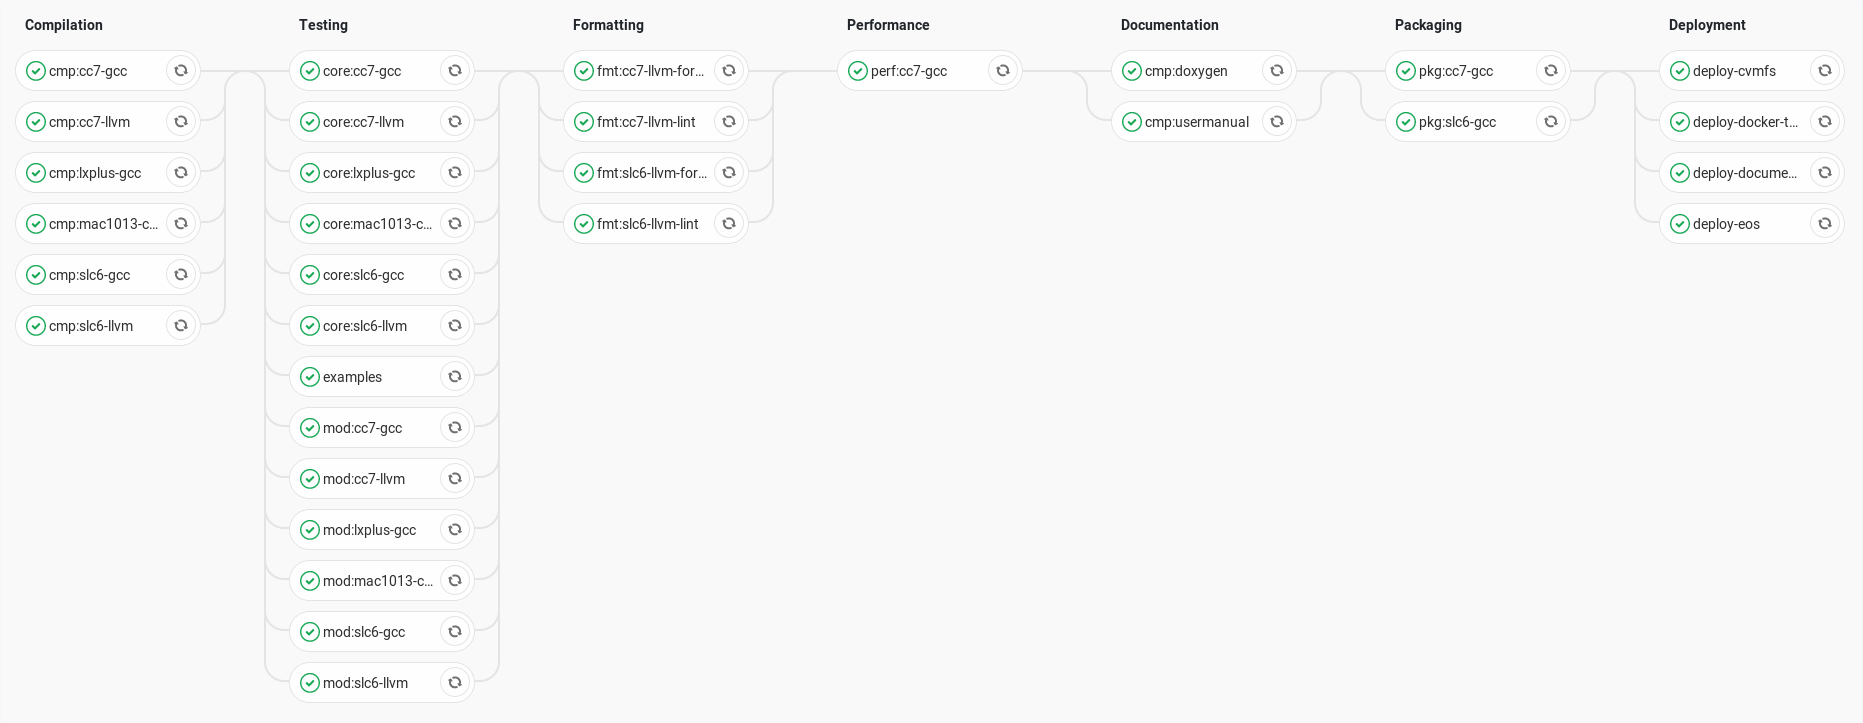
\includegraphics[width=\textwidth]{ci.png}
  \caption{Typical \apsq continuous integration pipeline with 34 jobs distributed over seven distinct stages. In this example, all jobs passed.}
  \label{fig:ci}
\end{figure}

The \textbf{compilation} stage builds the framework from the source on different platforms.
Currently, builds are performed on CentOS\,7, CentOS\,8, and macOS.
On Linux type platforms, the framework is compiled with recent versions of GCC and Clang, while the latest AppleClang is used on macOS.
The build is always performed with the default compiler flags enabled for the project:
\begin{verbatim}
    -pedantic -Wall -Wextra -Wcast-align -Wcast-qual -Wconversion
    -Wuseless-cast -Wctor-dtor-privacy -Wzero-as-null-pointer-constant
    -Wdisabled-optimization -Wformat=2 -Winit-self -Wlogical-op
    -Wmissing-declarations -Wmissing-include-dirs -Wnoexcept
    -Wold-style-cast -Woverloaded-virtual -Wredundant-decls
    -Wsign-conversion -Wsign-promo -Wstrict-null-sentinel
    -Wstrict-overflow=5 -Wswitch-default -Wundef -Werror -Wshadow
    -Wformat-security -Wdeprecated -fdiagnostics-color=auto
    -Wheader-hygiene
\end{verbatim}

The \textbf{testing} stage executes the framework system and unit tests described in Section~\ref{sec:tests}.
Different jobs are used to run different test types.
This allows to optimize the CI setup depending on the demands of the test to be executed.
All tests are expected to pass, and no code that fails to satisfy all tests will be merged into the repository.

The \textbf{formatting} stage ensures proper formatting of the source code using the \command{clang-format} and following the coding conventions defined in the \file{.clang-format} file in the repository.
In addition, the \command{clang-tidy} tool is used for ``linting'' of the source code.
This means, the source code undergoes a static code analysis in order to identify possible sources of bugs by flagging suspicious and non-portable constructs used.
Tests are marked as failed if either of the CMake targets \command{make check-format} or \command{make check-lint} fail.
No code that fails to satisfy the coding conventions and formatting tests will be merged into the repository.
Furthermore, also basic sanity checks are carried out on the CMake build framework code using \command{cmake-lint}.

The \textbf{performance} stage runs a longer simulation with several thousand events and measures the execution time.
This facilitates monitoring of the simulation performance, a failing job would indicate a degradation in speed.
These CI jobs run on dedicated machines with only one concurrent job as described in Section~\ref{sec:tests}.
Performance tests are separated into their own CI stage because their execution is time consuming and they should only be started once proper  formatting of the new code is established.

The \textbf{documentation} stage prepares this user manual as well as the Doxygen source code documentation for publication.
This also allows to identify e.g.\ failing compilation of the \LaTeX documents or additional files which accidentally have not been committed to the repository.

The \textbf{packaging} stage wraps the compiled binaries up into distributable tarballs for several platforms.
This includes adding all libraries and executables to the tarball as well as preparing the \file{setup.sh} script to prepare run-time dependencies using the information provided to the build system.
This procedure is described in more detail in Section~\ref{sec:packaging}.

Finally, the \textbf{deployment} stage is only executed for new tags in the repository.
Whenever a tag is pushed, this stages receives the build artifacts of previous stages and publishes them to the \apsq project website through the EOS file system~\cite{eos}. More detailed information on deployments is provided in the following.

\section{Automatic Deployment}

The CI is configured to automatically deploy new versions of \apsq and its user manual and code reference to different places to make them available to users.
This section briefly describes the different deployment end-points currently configured and in use.
The individual targets are triggered either by automatic nightly builds or by publishing new tags.
In order to prevent accidental publications, the creation of tags is protected.
Only users with \emph{Maintainer} privileges can push new tags to the repository.
For new tagged versions, all deployment targets are executed.

\subsection{Software deployment to CVMFS}
\label{sec:cvmfs}

The software is automatically deployed to CERN's VM file system (CVMFS)~\cite{cvmfs} for every new tag.
In addition, the \parameter{master} branch is built and deployed every night.
New versions are published to the folder \dir{/cvmfs/clicdp.cern.ch/software/allpix-squared/} where a new folder is created for every new tag, while updates via the \parameter{master} branch are always stored in the \dir{latest} folder.

The deployed version currently comprises all modules as well as the detector models shipped with the framework.
An additional \file{setup.sh} is placed in the root folder of the respective release, which allows to set up all runtime dependencies necessary for executing this version.
Versions both for CentOS\,7 and CentOS\,8 are provided.

The deployment CI job runs on a dedicated computer with a GitLab SSH runner.
Job artifacts from the packaging stage of the CI are downloaded via their ID using the script found in \dir{.gitlab/ci/download_artifacts.py}, and are made available to the \emph{cvclicdp} user which has access to the CVMFS interface.
The job checks for concurrent deployments to CVMFS and then unpacks the tarball releases and publishes them to the CLICdp experiment CVMFS space, the corresponding script for the deployment can be found in \dir{.gitlab/ci/gitlab_deployment.sh}.
This job requires a private API token to be set as secret project variable through the GitLab interface, currently this token belongs to the service account user \emph{ap2}.

\subsection{Documentation deployment to EOS}

The project documentation is deployed to the project's EOS space at \dir{/eos/project/a/allpix-squared/www/} for publication on the project website.
This comprises both the PDF and HTML versions of the user manual (subdirectory \dir{usermanual}) as well as the Doxygen code reference (subdirectory \dir{reference/}).
The documentation is only published for new tagged versions of the framework.

The CI jobs uses the \parameter{ci-web-deployer} Docker image from the CERN GitLab CI tools to access EOS, which requires a specific file structure of the artifact.
All files in the artifact's \dir{public/} folder will be published to the \dir{www/} folder of the given project.
This job requires the secret project variables \parameter{EOS_ACCOUNT_USERNAME} and \parameter{EOS_ACCOUNT_PASSWORD} to be set via the GitLab web interface.
Currently, this uses the credentials of the service account user \emph{ap2}.

\subsection{Release tarball deployment to EOS}

Binary release tarballs are deployed to EOS to serve as downloads from the website to the directory \dir{/eos/project/a/allpix-squared/www/releases}.
New tarballs are produced for every tag as well as for nightly builds of the \parameter{master} branch, which are deployed with the name \file{allpix-squared-latest-<system-tag>-opt.tar.gz}.

The files are taken from the packaging jobs and published via the \parameter{ci-web-deployer} Docker image from the CERN GitLab CI tools.
This job requires the secret project variables \parameter{EOS_ACCOUNT_USERNAME} and \parameter{EOS_ACCOUNT_PASSWORD} to be set via the GitLab web interface.
Currently, this uses the credentials of the service account user \emph{ap2}.

\section{Building Docker images}
\label{sec:build-docker}

New \apsq Docker images are automatically created and deployed by the CI for every new tag and as a nightly build from the \parameter{master} branch.
New versions are published to project Docker container registry~\cite{ap2-container-registry}.
Tagged versions can be found via their respective tag name, while updates via the nightly build are always stored with the \parameter{latest} tag attached.

The final Docker image is formed from two consecutive images with different layers of software added.
The \parameter{deps} image contains all build dependencies such as compilers, CMake, and git as well as the two main dependencies of the framework are ROOT6 and Geant4.
It derives from the latest Ubuntu LTS Docker image and can be build using the \file{etc/docker/Dockerfile.deps} file via the following commands:

\begin{verbatim}
$ docker build --file etc/docker/Dockerfile.deps            \
               --tag gitlab-registry.cern.ch/allpix-squared/\
               allpix-squared/allpix-squared-deps           \
              .
$ docker push gitlab-registry.cern.ch/allpix-squared/\
              allpix-squared/allpix-squared-deps
\end{verbatim}
This image is created manually and only updated when necessary, i.e.\ if major new version of the underlying dependencies are available.

\begin{warning}
  The dependencies Docker image should not be flattened with commands like

  \command{docker export <container id> | docker import - <tag name>}

  because it strips any \parameter{ENV} variables set or used during the build process. They are used to set up the ROOT6 and Geant4 environments. When flattening, their executables and data paths cannot be found in the final \apsq image.
\end{warning}

Finally, the latest revision of \apsq is built using the file \file{etc/docker/Dockerfile}.
This job is performed automatically by the continuous integration and the created containers are directly uploaded to the project's Docker registry.
\begin{verbatim}
$ docker build --file etc/docker/Dockerfile                                \
               --tag gitlab-registry.cern.ch/allpix-squared/allpix-squared \
              .
\end{verbatim}

A short summary of potential use cases for Docker images is provided in Section~\ref{sec:docker}.

\section{Tests}
\label{sec:tests}

The build system of the framework provides a set of automated tests which are executed by the CI to ensure proper functioning of the framework and its modules.
The tests can also be manually invoked from the build directory of \apsq with
\begin{verbatim}
$ ctest
\end{verbatim}
When executed by the CI, the results on passed and failed tests are automatically gathered and prominently displayed in merge requests along with the overall CI pipeline status.
This allows a quick identification of issues without having to manually search through the log of several CI jobs.

The different subcategories of tests described below can be executed or ignored using the \command{-E} (exclude) and \command{-R} (run) switches of the \command{ctest} program:
\begin{verbatim}
$ ctest -R test_performance
\end{verbatim}

The configuration of the tests can be found in the \dir{etc/unittests/test_*} directories of the repository and are automatically discovered by CMake.
CMake automatically searches for \apsq configuration files in the different directories and passes them to the \apsq executable~(cf.\ Section~\ref{sec:allpix_executable}).

Adding a new test is as simple as adding a new configuration file to one of the different subdirectories and specifying the pass or fail conditions based on the tags described in the following paragraphs.

\paragraph{Test Tags, Pass and Fail Conditions}

Test tags allow to influence the execution condition of the given test configuration, or to define a required condition for passing or failing the test.
These expressions are simply placed in the configuration file of the corresponding tests, a tag at the beginning of the line indicates which test tag the line corresponds to.
The following tags are available:

\begin{description}
  \item[Passing a test] The expression marked with the tag \parameter{#PASS} has to be found in the output in order for the test to pass. If the expression is not found, the test fails.
  \item[Failing a test] If the expression tagged with \parameter{#FAIL} is found in the output, the test fails. If the expression is not found, the test passes.
  \item[Depending on another test] The tag \parameter{#DEPENDS} can be used to indicate dependencies between tests. For example, the module test 09 described below implements such a dependency as it uses the output of module test 08-1 to read data from a previously produced \apsq data file.
  \item[Defining a timeout] For performance tests the runtime of the application is monitored, and the test fails if it exceeds the number of seconds defined using the \parameter{#TIMEOUT} tag.
  \item[Adding additional CLI options] Additional module command line options can be specified for the \parameter{allpix} executable using the \parameter{#OPTION} tag, following the format found in Section~\ref{sec:allpix_executable}. The \parameter{-o} flag will be added automatically. Multiple options can be supplied by repeating the \parameter{#OPTION} tag in the configuration file, only one option per tag is allowed. In exactly the same way options for the detectors can be set as well using the \parameter{#DETOPION} tag, where \parameter{-g} will be added automatically.
  For all other command line options to be passed to the executable, the \parameter{#CLIOPTION} can be used. Here, the complete flag and possible value needs to be passed, e.g.\ \parameter{-j9}.
  \item[Defining a test case label] Tests can be grouped and executed based on labels, e.g.\ for code coverage reports. Labels can be assigned to individual tests using the \parameter{#LABEL} tag.
\end{description}

Multiple pass or fail conditions can be separated by a semicolon or by adding multiple \parameter{#PASS} or \parameter{#FAIL} expressions.
It should however be noted that test passes or fails \emph{if any of these conditions is met}, i.e.\ the conditions are combined with a logical \parameter{OR}.
At least one pass or one fail conditions must be present in every test.

Pass and fail condition are not interpreted as regular expressions but relevant characters are automatically escaped.
This allows to directly copy corresponding lines form the log into the respective condition without manually creating a matching regular expression.
A noteworthy exception to this are line breaks.
To ease matching of multi-line expressions, the newline escape sequence \parameter{\n} of any test expression is automatically expanded to \parameter{[\r\n\t ]*} to match any new line, carriage return, tab and whitespace characters following the line break.

If no explicit fail conditions are specified, the test will fail if any \parameter{WARNING}, \parameter{ERROR} or \parameter{FATAL} appears in the output log unless it is already part of the pass condition.
For example, if a test is supposed to pass in case of an error provoked

\begin{minted}[frame=single,framesep=3pt,breaklines=true,tabsize=2,linenos]{bash}
(FATAL) [I:GeometryBuilderGeant4] Error during execution of run:
                                  Could not find a detector model of type 'missing_model'
                                  Please check your configuration and modules. Cannot continue.
\end{minted}

The full error message including the \parameter{FATAL} has to be provided as pass condition:

\begin{minted}[frame=single,framesep=3pt,breaklines=true,tabsize=2,linenos]{ini}
#PASS (FATAL) [I:GeometryBuilderGeant4] Error during execution of run:\nCould not find a detector model of type 'missing_model'
\end{minted}

If a test is expected to create multiple error or warning messages which cannot be matched with a single pass condition, the \parameter{#FAIL} parameter should be set explicitly to avoid matching the respective flags:

\begin{minted}[frame=single,framesep=3pt,breaklines=true,tabsize=2,linenos]{ini}
# This test created multiple WARNING messages, we exclude WARNING from the
# fail expression by explicitly defining it as FATAL only:
#PASS (ERROR) Multithreading disabled since the current module configuration does not support it
#FAIL FATAL
\end{minted}

\paragraph{Directory Variables in Tests}

Sometimes it is necessary to pass directories or file names as test input.
To facilitate this, the test files can contain variables which are replaced with the respective paths before being executed.
All variable names have to be enclosed in \parameter{@} symbols to be detected and parsed correctly.
Variables can be used both in test files and the auxiliary configuration files such as detector geometry definitions.

The following variables are available:

\begin{description}
  \item[\parameter{@TEST_DIRECTORY@}:] Directory in which the current test is executed, i.e. where all output files will be placed.
  \item[\parameter{@TEST_BASE_DIRECTORY@}:] Base directory under which all tests are being executed. This can be used to reference the output files from another test. it should be noted that the respective test has to be referenced using the \parameter{#DEPENDS} keyword to ensure that it successfully ran before.
  \item[\parameter{@PROJECT_SOURCE_DIR@}:] The root directory of the project. This can for example be used to call a script provided in the \dir{etc/scripts} directory of the repository.
\end{description}

The following example demonstrates the use of these variables.
A script is called before executing the test and an input file is expected:

\begin{minted}[frame=single,framesep=3pt,breaklines=true,tabsize=2,linenos]{ini}
[Allpix]
detectors_file = "detector.conf"

[DepositionReader]
file_name = "@TEST_DIRECTORY@/deposition.root"

#BEFORE_SCRIPT python @PROJECT_SOURCE_DIR@/etc/scripts/create_deposition_file.py --type a --detector mydetector
\end{minted}


% frequently asked question
\chapter{Frequently Asked Questions}
\label{ch:faq}

This chapter provides answers to some of the most frequently asked questions concerning usage, configuration and extension of the \apsq framework.

\section{Installation \& Usage}

\begin{description}
\item[What is the easiest way to use \apsq on CERN's LXPLUS?]
Central installations of \apsq on LXPLUS are provided via CVMFS for both supported LXPLUS operating systems, CERN CentOS\,7 and CentOS\,8. Please refer to Section~\ref{sec:cvmfs} for the details of how to access these installations.
\item[What is the quickest way to get a local installation of \apsq?]
The project provides ready-to-use Docker containers which contain all dependencies such as Geant4 and ROOT. Please refer to Section~\ref{sec:docker} for more information on how to start and use these containers.
\end{description}

\section{Configuration}
\begin{description}
\item[How do I run a module only for one detector?]
This is only possible for detector modules (which are constructed to work on individual detectors).
To run it on a single detector, one should add a parameter \parameter{name} specifying the name of the detector (as defined in the detector configuration file):
\begin{minted}[frame=single,framesep=3pt,breaklines=true,tabsize=2,linenos]{ini}
[ElectricFieldReader]
name = "dut"
model = "mesh"
file_name = "../example_electric_field.init"
\end{minted}
\item[How do I run a module only for a specific detector type?]
This is only possible for detector modules (which are constructed to work on individual detectors).
To run it for a specific type of detector, one should add a parameter \parameter{type} with the type of the detector model (as set in the detector configuration file by the \parameter{model} parameter):
\begin{minted}[frame=single,framesep=3pt,breaklines=true,tabsize=2,linenos]{ini}
[ElectricFieldReader]
type = "timepix"
model = "linear"
bias_voltage = -50V
depletion_voltage = -30V
\end{minted}
Please refer to Section~\ref{sec:module_instantiation} for more information.
\item[How can I run the exact same type of module with different settings?] This is possible by using the \parameter{input} and \parameter{output} parameters of a module that specify the messages of the module:
\begin{minted}[frame=single,framesep=3pt,breaklines=true,tabsize=2,linenos]{ini}
[DefaultDigitizer]
name = "dut0"
adc_resolution = 4
output = "low_adc_resolution"

[DefaultDigitizer]
name = "dut0"
adc_resolution = 12
output = "high_adc_resolution"
\end{minted}
By default, both the input and the output of module are messages with an empty name.
In order to further process the data, subsequent modules require the \parameter{input} parameter to not receive multiple messages:
\begin{minted}[frame=single,framesep=3pt,breaklines=true,tabsize=2,linenos]{ini}
[DetectorHistogrammer]
input = "low_adc_resolution"
name = "dut0"

[DetectorHistogrammer]
input = "high_adc_resolution"
name = "dut0"
\end{minted}
Please refer to Section~\ref{sec:objects_messages} for more information.
\item[How can I temporarily ignore a module during development?]
The section header of a particular module in the configuration file can be replaced by the string \parameter{Ignore}.
The section and all of its key/value pairs are then ignored.
Modules can also be excluded from the compilation process as explained in Section~\ref{sec:cmake_config}.
\item[Can I get a high verbosity level only for a specific module?]
Yes, it is possible to specify verbosity levels and log formats per module.
This can be done by adding the \parameter{log_level} and/or \parameter{log_format} key to a specific module to replace the parameter in the global configuration sections.

\item[Can I import an electric field from TCAD and use it for simulating propagation?]
Yes, the framework includes a tool to convert DF-ISE files from TCAD to an internal format which \apsq can parse.
More information about this tool can be found in Section~\ref{sec:tcad_electric_field_converter}, instructions to import the generated field are provided in Section~\ref{sec:module_electric_field}.
\end{description}

\section{Detector Models}
\begin{description}
\item[I want to use a detector model with one or several small changes, do I have to create a whole new model for this?] No, models can be specialized in the detector configuration file.
To specialize a detector model, the key that should be changed in the standard detector model, e.g.\ like \parameter{sensor_thickness}, should be added as key to the section of the detector configuration (which already contains the position, orientation and the base model of the detector).
Only parameters in the header of detector models can be changed.
If support layers should be changed, or new support layers are needed, a new model should be created instead.
Please refer to Section~\ref{sec:detector_models} for more information.
\end{description}

\section{Data Analysis}
\begin{description}
\item[How do I access the history of a particular object?]
Many objects can include an internal link to related other objects (for example \parameter{getPropagatedCharges} in the \parameter{PixelCharge} object), containing the history of the object (thus the objects that were used to construct the current object).
These referenced objects are stored as special ROOT pointers inside the object, which can only be accessed if the referenced object is available in memory.
In \apsq this requirement can be automatically fulfilled by also binding the history object of interest in a module.
During analysis, the tree holding the referenced object should be loaded and pointing to the same event entry as the object that requests the reference.
If the referenced object can not be loaded, an exception is thrown by the retrieving method.
Please refer to Section~\ref{sec:objhistory} for more information.
\item[How do I access the Monte Carlo truth of a specific PixelHit?]
The Monte Carlo truth is part of the history of a PixelHit.
This means that the Monte Carlo truth can be retrieved as described in the question above.
Because accessing the Monte Carlo truth of a PixelHit is quite a common task, these references are stored directly for every new object created.
This allows to retain the information without the necessity to keep the full object history including all intermediate steps in memory.
Please refer to Section~\ref{sec:objhistory} for more information.
\item[How do I find out, which Monte Carlo particles are primary particles and which have been generated in the sensor?]
The Monte Carlo truth information is stored per-sensor as MCParticle objects. Each MCParticle stores, among other information, a reference to its parent. Particles which have entered the sensor from the outside world do not have parent MCParticles in the respective sensor and are thus primaries.

Using this approach it is possible, to e.g.\ treat a secondary particle produced in one detector as primary in a following detector.

Below is some pseudo-code to filter a list of MCParticle objects for primaries based on their parent relationship:

\begin{minted}[frame=single,framesep=3pt,breaklines=true,tabsize=2,linenos]{c++}
// Collect all primary particles of the event:
std::vector<const MCParticle*> primaries;

// Loop over all MCParticles available
for(auto& mc_particle : my_mc_particles) {
    // Check for possible parents:
    if(mc_particle.getParent() != nullptr) {
        // Has a parent, thus was created inside this sensor.
        continue;
    }

    // Has no parent particles in this sensor, add to primary list.
    primaries.push_back(&mc_particle);
}
\end{minted}

A similar function is used e.g.\ in the DetectorHistogrammer module to filter primary particles and create position-resolved graphs.
Furthermore, the PixelHit object provides two member functions to access Monte Carlo particles, one which returns all known particles, \parameter{getMCParticles()}, and a second function called \parameter{getPrimaryMCParticles()} which already performs the above filtering and only returns primary particle references.
\item[How do I access data stored in a file produced with the ROOTObjectWriter from an analysis script?]
\apsq uses ROOT trees to directly store the relevant \CPP objects as binary data in the file. This retains all information present during the simulation run, including relations between different objects such as assignment of Monte Carlo particles.
In order to read such a data file in an analysis script, the relevant \CPP library as well as its header have to be loaded.

In ROOT this can be done interactively by loading a data file, the necessary shared library objects and a macro for the analysis:

\begin{minted}[frame=single,framesep=3pt,breaklines=true,tabsize=2,linenos]{bash}
$ root -l data_file.root
root [1] .L ~/path/to/your/allpix-squared/lib/libAllpixObjects.so
root [2] .L analysisMacro.C+
root [3] readTree(_file0, "detector1")
\end{minted}

A simple macro for reading DepositedCharges from a file and displaying their position is presented below:

\begin{minted}[frame=single,framesep=3pt,breaklines=true,tabsize=2,linenos]{c++}
#include <TFile.h>
#include <TTree.h>

// FIXME: adapt path to the include file of APSQ installation
#include "/path/to/your/allpix-squared/DepositedCharge.hpp"

// Read data from tree
void readTree(TFile* file, std::string detector) {

    // Read tree of deposited charges:
    TTree* dc_tree = static_cast<TTree*>(file->Get("DepositedCharge"));
    if(!dc_tree) {
        throw std::runtime_error("Could not read tree");
    }

    // Find branch for the detector requested:
    TBranch* dc_branch = dc_tree->FindBranch(detector.c_str());
    if(!dc_branch) {
        throw std::runtime_error("Could not find detector branch");
    }

    // Allocate object vector and link to ROOT branch:
    std::vector<allpix::DepositedCharge*> deposited_charges;
    dc_branch->SetObject(&deposited_charges);

    // Go through the tree event-by-event:
    for(int i = 0; i < dc_tree->GetEntries(); ++i) {
        dc_tree->GetEntry(i);
        // Loop over all deposited charge objects
        for(auto& charge : deposited_charges) {
            std::cout << "Event " << i << ": "
                      << "charge = " << charge->getCharge() << ", "
                      << "position = " << charge->getGlobalPosition()
                      << std::endl;
        }
    }
}

\end{minted}
A more elaborate example for a data analysis script can be found in the \dir{tools} directory of the repository and in Section~\ref{sec:root_analysis_macros} of this user manual.
Scripts written in both \CPP and in Python are provided.

\item[How can I convert data from the ROOTObject format to other formats?]
Since the ROOTObject format is the native format of \apsq, the stored data can be read into the framework again.
To convert it to another format, a simple pseudo-simulation setup can be used, which reads in data with one module and stores it with another.

In order to convert for example from ROOTObjects to the data format used by the Corryvreckan reconstruction framework, the following configuration could be used:
\begin{minted}[frame=single,framesep=3pt,breaklines=true,tabsize=2,linenos]{ini}
[Allpix]
number_of_events = 999999999
detectors_file = "telescope.conf"
random_seed_core = 0

[ROOTObjectReader]
file_name = "input_data_rootobjects.root"

[CorryvreckanWriter]
file_name = "output_data_corryvreckan.root"
reference = "mydetector0"
\end{minted}
\end{description}

\section{Development}
\begin{description}
\item[How do I write my own output module?]
An essential requirement of any output module is its ability to receive any message of the framework.
This can be implemented by defining a private \command{filter} function for the module as described in Section~\ref{sec:objects_messages}.
This function will be called for every new message dispatched within the framework, and should contain code to decide whether to discard or cache a message for processing.
Heavy-duty tasks such as handling data should not be performed in the \command{filter} routine, but deferred to the \command{run} function of the respective output module.
The \command{filter} function should only decide whether to keep a message for processing or to discard it before the \command{run} function.

\item[How do I process data from multiple detectors?]
When developing a new \apsq module which processes data from multiple detectors, e.g.\ as the simulation of a track trigger module, this module has to be of type \emph{unique} as described in Section~\ref{sec:module_manager}.
As a \emph{detector} module, it would always only have access to the information linked to the specific detector is has been instantiated for.
The module should then request all messages of the desired type using the messenger call \command{bindMulti} as described in Section~\ref{sec:objects_messages}.
For \emph{PixelHit} messages, an example code would be:

\begin{minted}[frame=single,framesep=3pt,breaklines=true,tabsize=2,linenos]{c++}
TrackTriggerModule(Configuration&, Messenger* messenger, GeometryManager* geo_manager) {
    messenger->bindMulti<MCTrackMessage>(this, MsgFlags::NONE);
}
std::vector<std::shared_ptr<PixelHitMessage>> messages;
\end{minted}
The correct detectors have then to be selected in the \command{run} function of the module implementation.
\item[How do I calculate an efficiency in a module?]
Calculating efficiencies always requires a reference.
For hit detection efficiencies in \apsq, this could be the Monte Carlo truth information available via the \emph{MCParticle} objects.
Since the framework only runs modules, if all input message requirements are satisfied, the message flags described in Section~\ref{sec:messageflags} have to be set up accordingly.
For the hit efficiency example, two different message types are required, and the Monte Carlo truth should always be required (using \command{MsgFlags::REQUIRED}) while the \emph{PixelHit} message should be optional:
\begin{minted}[frame=single,framesep=3pt,breaklines=true,tabsize=2,linenos]{c++}
MyModule::MyModule(Configuration& config, Messenger* messenger, std::shared_ptr<Detector> detector)
    : Module(config, detector), detector_(std::move(detector)) {

    // Bind messages
    messenger->bindSingle<PixelHitMessage>(this);
    messenger->bindSingle<MCParticleMessage>(this, MsgFlags::REQUIRED);
}
\end{minted}
\end{description}

\section{Miscellaneous}
\begin{description}
\item[How can I produce nicely looking drift-diffusion line graphs?]
The GenericPropagation module offers the possibility to produce line graphs depicting the path each of the charge carrier groups have taken during the simulation. This is a very useful way to visualize the drift and diffusion along field lines.

An optional parameter allows to reduce the lines drawn to those charge carrier groups which have reached the sensor surface to provide some insight into where from the collected charge carriers originate and how they reached the implants.
One graph is written per event simulated, usually this option should thus only be used when simulating one or a few events but not during a production run.

In order to produce a precise enough line graph, the integration time steps have to be chosen carefully - usually finer than necessary for the actual simulation. Below is a set of settings used to simulate the drift and diffusion in a high resistivity CMOS silicon sensor.
Settings of the module irrelevant for the line graph production have been omitted.

\begin{minted}[frame=single,framesep=3pt,breaklines=true,tabsize=2,linenos]{ini}
[GenericPropagation]
charge_per_step = 5
timestep_min = 1ps
timestep_max = 5ps
timestep_start = 1ps
spatial_precision = 0.1nm

output_linegraphs = true
output_plots_step = 100ps
output_plots_align_pixels = true
output_plots_use_pixel_units = true

# Optional to only draw charge carrier groups which reached the implant side:
# output_plots_lines_at_implants = true
\end{minted}

\begin{figure}[tbp]
    \centering
  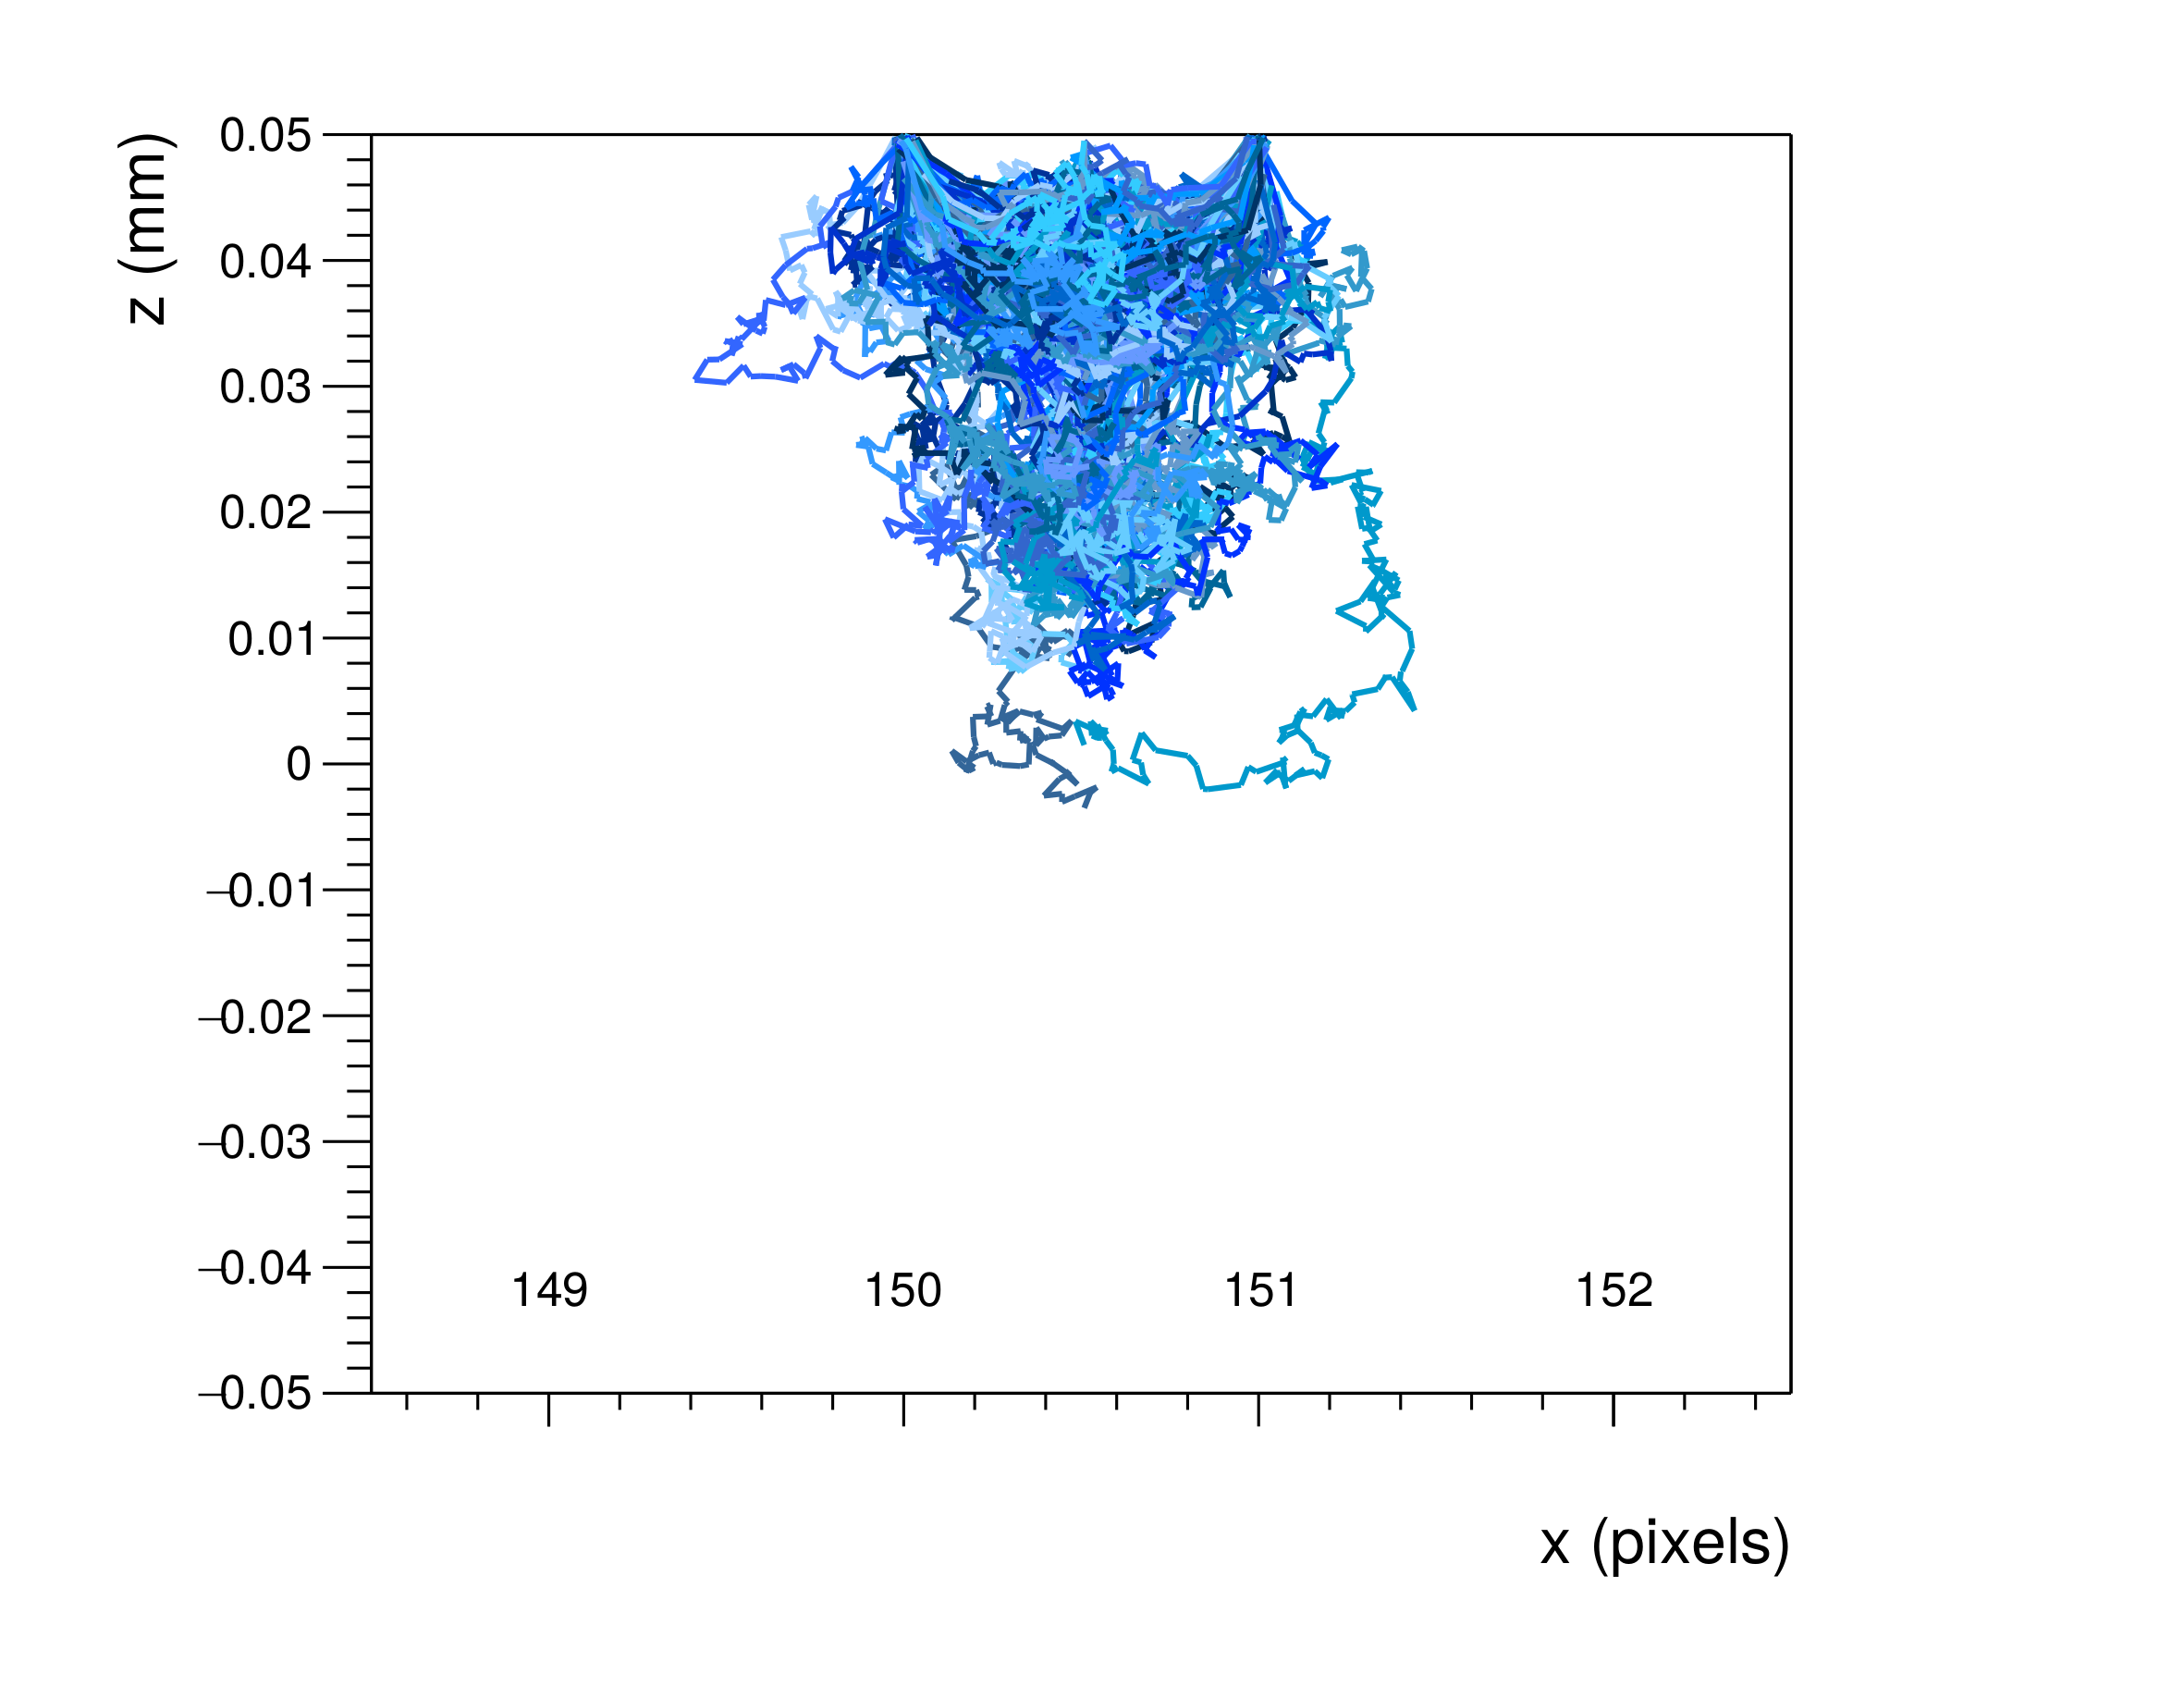
\includegraphics[width=0.7\textwidth]{linegraph_hrcmos_collected.png}
  \caption{Drift and diffusion visualization of charge carrier groups being transported through a high-resistivity CMOS silicon sensor. The plot shows the situation after an integration time of \SI{20}{\nano \second}, only charge carrier groups which reached the implant side of the sensor are drawn.}
  \label{fig:linegraph}
\end{figure}

With these settings, a graph of similar precision to the one presented in Figure~\ref{fig:linegraph} can be produced.
The required time stepping size and number of output plot steps varies greatly with the sensor and its applied electric field.
The number of charge carriers per group can be used to vary the density of lines drawn. Larger groups result in fewer lines.
\end{description}

\todo{Add more questions}


% additional tools and resources
\chapter{Additional Tools \& Resources}
\label{ch:additional_tools_resources}

This chapter briefly describes tools provided with the \apsq framework, which might be re-used in new modules or in standalone code.

\section{Framework Tools}

The following tools are part of the \apsq framework and are located in the \dir{src/tools} directory.
They are intended as centralized components which can be shared between different modules rather than independent tools.

\subsection{ROOT and Geant4 utilities}
\label{sec:root_and_geant4_utilities}
The framework provides a set of methods to ease the integration of ROOT and Geant4 in the framework.
An important part is the extension of the custom conversion \texttt{to\_string} and \texttt{from\_string} methods from the internal string utilities (see Section~\ref{sec:string_utilities}) to support internal ROOT and Geant4 classes.
This allows to directly read configuration parameters to these types, making the code in the modules both shorter and cleaner.
In addition, more conversions functions are provided together with other useful utilities such as the possibility to display a ROOT vector with units and a thin wrapper for thread-safe ROOT histograms.

\subsection{Geant4 Interface}
\label{sec:geant4_interface}
The framework provides an interfacing library with Geant4 that provides alternative run managers to be used by modules interested in using Geant4 as follows:
\begin{enumerate}
\item \texttt{MTRunManager}: A run manager that can only be used in parallel. Internally, it creates thread-local managers to handle operations for each calling thread independently. It also maintain a stable seed distribution mechanism to ensure results are the same regardless of the number of threads that used the manager in parallel.
\item \texttt{RunManager}: A run manager that can not be used in parallel. It uses the same seeding mechanism as the multi-threaded version so they can be used interchangeably depending on whether multi-threading is enabled or not.
\end{enumerate}

The DepositionGeant4 module uses \texttt{MTRunManager} to be able to call the \texttt{BeamOn} method in parallel thus benefiting from the multi-threading feature while the VisualizationGeant4 module uses \texttt{RunManager} to be able to visualize the particles passage through the detectors.

\subsection{Runge-Kutta integrator}
A fast Eigen-powered~\cite{eigen3} Runge-Kutta integrator is provided as a tool to numerically solve differential equations~\cite{fehlberg}.
The Runge-Kutta integrator is designed in a generic way and supports multiple methods using different tableaus.
It allows to integrate a system of equations in several steps with customizable step size.
The step size can also be updated during the integration depending on the error of the Runge-Kutta method (if a tableau with error estimation is used).

The GenericPropagation module uses Runge-Kutta integrator with the Runge-Kutta-Fehlberg method (RK5 tableau).
After the integrator has been created with the initial position of the charge carrier to be transported, the \command{step()} function allows to advance the simulation to the next step.
\begin{minted}[frame=single,framesep=3pt,breaklines=true,tabsize=2,linenos]{c++}
// Define lambda functions to compute the charge carrier velocity at each step
std::function<Eigen::Vector3d(double, Eigen::Vector3d)> carrier_velocity =
    [&](double, Eigen::Vector3d cur_pos) -> Eigen::Vector3d {...};

// Create the Runge-Kutta solver with a RK5 tableau, the carrier velocity function to be used
// as well as the initial timestep and position of the charge carrier
auto runge_kutta = make_runge_kutta(tableau::RK5, carrier_velocity, initial_timestep, position);

// Advance one step with the solver:
auto step = runge_kutta.step();
\end{minted}

The \command{getValue()} and \command{setValue()} methods allow to retrieve, alter and update the position, e.g. to include additional displacements from diffusion processes.

\subsection{Field Data Parser}
A field parser tool is provided, which parses files stored in the INIT or APF file formats and returns field data on a three-dimensional grid.
The number of field components per grid point is configurable via the constructor argument, e.g. \parameter{FieldQuantity::VECTOR} for a vector field or \parameter{FieldQuantity::SCALAR} for a scalar field map.
The parsed field data is cached internally by the class, and if a file is requested a second time, the cached field is returned.
In conjunction with a static instance of the field parser class in a module, this allows to share field data across multiple module instances.

\begin{minted}[frame=single,framesep=3pt,breaklines=true,tabsize=2,linenos]{c++}
class MyVectorFieldModule(...) : Module(...) {
private:
    void some_function(std::string canonical_path);
    // Define static field parser instance
    static FieldParser<double> field_parser_;
}

// Create static instance of field parser in the translation unit:
FieldParser<double> MyVectorFieldModule::field_parser_(FieldQuantity::VECTOR);

void MyVectorFieldModule::some_function(std::string canonical_path) {
    // Get vector field from file:
    auto field_data = field_parser_.getByFileName(canonical_path, "V/cm");
}
\end{minted}

For the INIT format, the \command{getByFileName()} function of the parser takes the units in which the field data should be interpreted, and they are automatically converted to the framework base units described in Section~\ref{sec:config_values}. Fields in the APF format are always stored in framework base units and do not require conversion.
The file path provided to the field parser should always be canonical, if the file is not found or cannot be parsed, a \command{std::runtime_error} exception is thrown.

The type of field data to be parsed is automatically deduced from the file content by checking for binary or ASCII text
The field parser determines whether a file is text or binary by checking the first few bytes in the file.
If every byte in that part of the file is non-null, the parser considers the file to be text and reads it as INIT file; otherwise it considers the file to be binary and parses the field as APF data.

\inputmd{tools/mesh_converter.tex}
% FIXME This label is not required to bind correctly
\label{sec:tcad_electric_field_converter}

\inputmd{tools/root_analysis_macros.tex}
% FIXME This label is not required to bind correctly
\label{sec:root_analysis_macros}


\backmatter

% acknowledgements to all contributors etc
\chapter{Acknowledgments}

\apsq has been developed and is maintained by

\begin{itemize}
\item Koen Wolters, (CERN)
\item Daniel Hynds, Nikhef
\item Paul Schütze, DESY
\item Simon Spannagel, DESY
\end{itemize}

The following authors, in alphabetical order, have contributed to \apsq:

\begin{itemize}
\item Mohamed Moanis Ali, Free University of Bozen-Bolzano
\item Mathieu Benoit, BNL
\item Thomas Billoud, Université de Montréal
\item Tobias Bisanz, CERN
\item Koen van den Brandt, Nikhef
\item Liejian Chen, Institute of High Energy Physics Beijing
\item Katharina Dort, University of Gie\ss en
\item Neal Gauvin, Université de Genève
\item Lennart Huth, DESY
\item Maoqiang Jing, University of South China, Institute of High Energy Physics Beijing
\item Moritz Kiehn, Université de Genève
\item Salman Maqbool, CERN Summer Student
\item Sebastien Murphy, ETHZ
\item Andreas Matthias Nürnberg, KIT
\item Sebastian Pape, TU Dortmund University
\item Marko Petric, CERN
\item Nashad Rahman, The Ohio State University
\item Edoardo Rossi, DESY
\item Andre Sailer, CERN
\item Enrico Jr. Schioppa, Unisalento and INFN Lecce
\item Sanchit Sharma, Kansas State University
\item Xin Shi, Institute of High Energy Physics Beijing
\item Viktor Sonesten, GSOC18 Student
\item Ondrej Theiner, Charles University
\item Annika Vauth, University of Hamburg
\item Mateus Vicente Barreto Pinto, CERN
\item Andy Wharton, Lancaster University
\item Morag Williams, University of Glasgow
\end{itemize}

The authors would also like to express their thanks to the developers of AllPix~\cite{ap1wiki,ap1git}.


\cleardoublepage
\phantomsection
\addreferencesline
\printbibliography

\end{document}
